% !TeX root = main.tex
%%%%%%%%%%%%%%%%%%%%%%%%% PREAMBLE %%%%%%%%%%%%%%%%%%%%%%%%%%%%%%%%
%%%%%%%%%%%%%%%%%%%%%%%% BASIC DOCUMENT SETUP %%%%%%%%%%%%%%%%%%%%%
\documentclass[a4paper]{report}
\usepackage[utf8]{inputenc}
\usepackage[english]{babel}

%%%%%%%%%%%%%%%%%%%%%%%%%% PACKAGES %%%%%%%%%%%%%%%%%%%%%%%%%%%%%%%
\usepackage{datetime}
\usepackage{datenumber}
\usepackage{parskip}
\usepackage{forest}
\usepackage{svg}        % makes it possible to use svg files
\usepackage{graphics}
\usepackage{multicol}
\usepackage{icomma}
\usepackage{microtype}  % microscopic typography refinement
\usepackage{lastpage}   % used to reference last page in footer
\usepackage{fancyhdr}   % Header
\usepackage{tcolorbox}
\usepackage{quiver}
\usepackage{amssymb}
\usepackage[Bjornstrup]{fncychap}
\usepackage[titles]{tocloft}
\usepackage{amsmath}    % mathematics for matrices and more
\usepackage{amsfonts}
\usepackage{csquotes}
\usepackage{morewrites}

\usepackage{tikz}
\usetikzlibrary{calc}   % position og tikz labels
\usetikzlibrary{arrows.meta}
\usetikzlibrary{decorations.pathreplacing,calligraphy}

\usepackage{float}
\usepackage{pgfplots}
\pgfplotsset{compat=1.17}
\usepackage{xcolor}
\definecolor{blueplot}{RGB}{60, 64, 198}
\definecolor{yellowplot}{RGB}{255, 211, 42}
\definecolor{redplot}{RGB}{255, 63, 52}
\definecolor{greenplot}{RGB}{5, 196, 107}
\definecolor{greyplot}{RGB}{72, 84, 96}

\usepackage{siunitx}
\sisetup{%quotient-mode=fraction,
		output-decimal-marker = {,},
		per-mode = fraction,
		separate-uncertainty = true,
		multi-part-units=single,
		exponent-product = \cdot,
		range-phrase=--}
		
\usepackage{minted} % Syntax highlighting 
%\usemintedstyle{monokai}
\setminted[]{breaklines, 
    breakafter=d,
    frame=lines,
    framesep=2mm,
    baselinestretch=1.2,
    fontsize=\footnotesize,
    tabsize=4,
    linenos}


\makeatletter
\renewcommand\@makefnmark{\textsuperscript{[\@thefnmark]}}
\renewcommand\@makefntext[1]{\textsuperscript{[\@thefnmark]}\enspace #1}
\makeatother

\usepackage[hidelinks, linktoc=all]{hyperref} % links, references, \ref{...}
\hypersetup{
    colorlinks = true,
    linkcolor = blue,
    citecolor = blue,
    urlcolor = blue
}
\urlstyle{same}

\usepackage{todonotes}

\usepackage{subcaption}

\usepackage{forest}

\usepackage{lipsum}  

\usepackage{wrapfig}

\usepackage[export]{adjustbox}


\usepackage[pdf]{graphviz}

%%% Helper code for Overleaf's build system to
%%% automatically update output drawings when
%%% code in a \digraph{...} is modified
\usepackage{xpatch}
\makeatletter
\newcommand*{\addFileDependency}[1]{% argument=file name and extension
  \typeout{(#1)}
  \@addtofilelist{#1}
  \IfFileExists{#1}{}{\typeout{No file #1.}}
}
\makeatother
\xpretocmd{\digraph}{\addFileDependency{#2.dot}}{}{}

\usepackage[block=ragged, sorting=nyt, style=authoryear-ibid, backend=biber]{biblatex}
\setlength\bibitemsep{1.5\itemsep}
\addbibresource{mybib.bib}

%%%%%%%%%%%%% ACTUAL VISIBLE CONTENT %%%%%%%%%%%%%%%%%%%%%%%%%%%%%%
\begin{document}
\begin{titlepage}
    \begin{centering}
    \vspace*{-20px}\large Department of Mathematics \& Computer Science\\
    University of Southern Denmark $|$ IMADA \\
    \today \\
    
    \vspace{\fill}
    
    \huge{\bf  Capture the Flag Platform} \\
    \Large{\bf SPDM801: Master's Thesis}
    
    \vspace{\fill}
    
    \begin{minipage}{0.45\textwidth} 
    \begin{flushleft}
        \Large
        \textit{Author}\\
        KIAN BANKE LARSEN\\
        kilar20@student.sdu.dk
    \end{flushleft}
    \end{minipage}
    
    \vspace{\fill}
    
    \begin{minipage}{0.45\textwidth}
    \begin{flushleft}
        \Large
        \textit{Supervisor}\\
        Jacopo Mauro\\
        Professor
    \end{flushleft}
    \end{minipage}
    
    \vspace{\fill}
    
    \includesvg[width=.4\textwidth]{template/SDU.svg}
    
    \vspace*{0.1cm}
    
    \end{centering}
    
    \thispagestyle{empty}
\end{titlepage}

\begin{abstract}
\paragraph{English}

\paragraph{Danish}
\end{abstract}

\chapter*{Acknowledgements}
\thispagestyle{empty}
\clearpage

\pagenumbering{roman}

{ \hypersetup{hidelinks} \tableofcontents \addtocontents{toc}{\vskip-40pt}}

\newpage
\pagenumbering{arabic}
\setcounter{page}{1}

\chapter{Introduction}
Digitalization has become an integral part of our lives. As technology continues to evolve, so do the challenges associated with it. One of the most pressing issues in today's digital landscape is cybersecurity, as it is part of \textit{Europe's digital targets for 2030} \Parencite{europe_digital_decade}. The Agency for Digital Government marks Denmark as a digital frontrunner \Parencite{danish_digital_journey}. The strong digital infrastructure we have today has been achieved through more than 20 years of close collaboration amongst Danish IT companies, the Danish national government municipalities and regions. Examples of such IT companies are KMD, EG and Netcompany. The digital infrastructure offers automation of repetitive manual tasks and accessibility to information and services. While automation minimizes the risk of human errors, the increased use of software libraries and expanded accessibility also enlarge the attack surface.

With the increasing number of cyber threats and attacks, organizations are constantly seeking ways to enhance their security measures and protect their sensitive data. This has led to a growing demand for educated cybersecurity professionals who can proactively identify and mitigate risks. Such know-how is partly taught from workshops, books, talks etc., but an important key ingredient is practical experience. One way to achieve this is through the use of a competitive Capture the Flag (CTF) game. CTFs are a kind of computer security competition. Two kinds of CTF competitions exist \Parencite{ctf_overview}: 

\begin{itemize}
    \item Jeopardy revolve around a set of challenges provided by the competition organizers. They are mainly focusing on exploiting a system in order to reveal a small piece of text or ``flag''. 
    \item Attack \& Defense is a kind of CTF where the participants are given a set of vulnerable server software. The goal is to attack the other teams' servers while defending their own. A successful attack is one that retrieves a flag. Its purpose is to simulate digital warfare.
\end{itemize}

This thesis will not go into detail regarding the CTF challenges themselves, but rather focus on the infrastructure and architecture of a platform hosting such challenges. We will though provide some very simplistic Jeopardy challenges to demonstrate the platform's capabilities.

\section{Motivation}
The motivation behind this thesis is to develop a CTF platform tailored for educational purposes, particularly for Computer Science bachelor's students at the University of Southern Denmark. The platform was initially designed to be hosted on UCloud \Parencite{SDUCloud}, a cloud service managed by the University of Southern Denmark and supported by servers from Aarhus University. However, due to the missing support for hardware virtualization, we decided to migrate the platform to Hetzner \Parencite{Hetzner}. To our surprise Hetnzer does not support hardware virtualization either \Parencite{hetzner_nested_virtualization}, forcing us to use the Google Cloud Platform (GCP). This change in setting enabled us to eliminate certain complexities that were otherwise imposed by using UCloud, as detailed in Section \ref{sec:architecture}. UCloud was initially chosen because of its cost-effectiveness and the fact that it is a service provided by the university.

Although this Master's Thesis was developed independently, it is essential to acknowledge the contributions of the individuals who played a role in the project. The group composition was as follows: Henrik Rossen Jakobsen, a former Master's student, began his Thesis in January 2024. His initial research focused on analyzing different CTF platforms by comparing their strengths and weaknesses. This analysis established a set of requirements for the platform to be developed. I joined Henrik in September 2024 to assist in the platform's development. Due to the limitations of UCloud, Matteo Trentin, a PhD student, joined the project to establish a distributed Kubernetes cluster on both UCloud and GCP. Following this, we worked independently while contributing features to a unified platform. We all share the same supervisor, Jacopo Mauro, who provided guidance and support throughout the project.

By reading Henrik's Thesis, I was able to gain insights into the main state-of-the-art competitor, namely Haaukins. This platform is also used to host the De Danske Cybermesterskaber (DDC). The drawbacks of the platform is that it is complicated to deploy due to limited documentation and manual steps, and there is no way to check the validity of a challenge without creating a CTFd event. Additionally, containers are a widely used solution for deploying challenges. However, they carry the risk of container escape, where an attacker could exploit a vulnerability to gain access to the host system. This risk is heightened in the context of CTF competitions, as challenges may deliberately include vulnerabilities -- we have mitigated this risk by using Virtual Machines (VMs) instead of containers.

\section{Contributions} 

\begin{figure}
    \centering
    \includesvg[width=1\textwidth]{../assets/images/wordcloud.svg}
    \caption{Word cloud generated from technologies applied in this thesis.}
    \label{fig:wordcloud}
\end{figure}

\section{Structure} 

The project files and documentation are available at \url{https://kianbankelarsen.github.io/CTF-Platform/}, along with additional related resources, all of which can be accessed through this URL.

This report was prepared with the assistance of generative AI tools such as Edge Copilot and GitHub Copilot, specifically for linguistic refinement and error correction purposes.

\chapter{State of the Art}

This chapter provides an overview of the key concepts, tools, and technologies needed to develop a scalable and reliable CTF platform. Building such a platform requires understanding the current approaches and learning from past implementations to make the best use of open-source software (OSS). By looking into established methods and tools, this chapter helps guide the decisions made throughout the project.

Topics covered include Infrastructure as Code (IaC) for easier deployment, Dynamic Storage Provisioning for storage management and backup, Private Key Infrastructure (PKI) for data integrity, and Identity and Access Management (IAM) for access control. These areas and others form the basis for creating a secure and efficient CTF platform.

\section{Infrastructure as Code}

Infrastructure as Code (IaC) is a modern approach to provision and configure resources. IaC is desirable because it offers consistency and repeatability, reducing the risk of human error and ensuring that the infrastructure is always in a known state. The critical importance of such reliability is underscored by incidents like the Knight Capital Group's failed deployment, which resulted in the loss of nearly \$400 million within just 45 minutes \Parencite{seven2014knightmare}. Additional benefits of IaC include version control and documentation. Version control allows for easier disaster recovery, as the entire infrastructure can be restored to a previous state if needed. Documentation is automatically generated, as the code itself serves as documentation. 

Tools like Pulumi and Terraform, which only require interface implementation, inherently support both Cloud-Native and Multi-Cloud environments. The cloud-agnostic nature of the code simplifies migration between clouds. Ansible, an OSS licensed under Apache License 2.0 \Parencite{ansible_license}, is a complementing tool to Pulumi and Terraform. Ansible specializes in configuration management and software provisioning. It uses YAML-based playbooks to install software and configure servers. Pulumi and Terraform excel at provisioning servers and setting up cloud infrastructure, while Ansible handles fine-tuning and ongoing maintenance. Together, these tools enable full-stack automation.

IaC is not limited to the tools mentioned. Vagrant, Chef, and Puppet also belong under the IaC umbrella \Parencite{spacelift_iac_tools}. Idempotence is essential, ensuring consistent results regardless of repeated execution.

\subsection{Pulumi versus Terraform}
Pulumi and Terraform are very similar tools, but they differ in their approach to defining infrastructure. Terraform uses a domain-specific language (DSL) called HashiCorp Configuration Language (HCL), which is declarative. This means that you describe the desired state of your infrastructure, and Terraform figures out how to achieve that state. Pulumi, on the other hand, uses general-purpose programming languages like TypeScript, Python, Go, and C\# \Parencite{pulumi_vs_terraform}. This allows for more flexibility and the ability to use existing libraries and tools. Thereby, Pulumi is primarily declarative, but it incorporates imperative capabilities to include procedural logic alongside infrastructure definitions.

Terraform began its journey in 2014 \Parencite{hashicorpTerraform}, laying the foundation for Infrastructure as Code (IaC) tools, while Pulumi entered the scene in 2017 \Parencite{pulumiAbout}. Pulumi remains open-source software (OSS), distributed under the Apache 2.0 license \Parencite{pulumiLicense2025}. In 2024, IBM's acquisition of HashiCorp resulted in Terraform transitioning to closed-source software (CSS). In response, OpenTofu emerged as a fork of Terraform \Parencite{opentofu}, ensuring the continuation of open-source alternatives. OpenTofu is licensed under the Mozilla Public License 2.0 \Parencite{opentofuLicense2025}. In order to transition users from Terraform to Pulumi, Pulumi provides software to convert template files from HCL into Pulumi programs \Parencite{pulumiMigration2025}.

The functionalities offered by Pulumi and Terraform are largely similar, though there are some technical distinctions. While this project does not require advanced features provided by either tool, we do benefit from Pulumi's capability to support encrypted secrets. This facilitates seamless secret management both locally and in production environments, eliminating the need for paid external secret vaults \Parencite{pulumi_vs_terraform}. Additionally, Pulumi provides dynamic provider support -- a feature not available in Terraform. Conversely, Terraform supports Policy as Code, which is not offered by Pulumi. Pulumi can adapt any Terraform provider, enabling the management of all infrastructure supported by Terraform.

\subsection{Pipelines}
Pipelines are not typically considered IaC tools but are often used alongside them to automate the deployment of applications and infrastructure. While IaC defines infrastructure using code, pipelines focus on workflows, such as Continuous Integration and Continuous Deployment (CI/CD). Unlike the discussed IaC tools, which are cloud-agnostic, pipelines are often closely tied to specific cloud providers. This can make migrations more challenging, as many pipelines rely on proprietary domain-specific languages (DSL) unique to their platforms. Examples of popular pipelines include those from GitLab, GitHub, Azure DevOps, and open-source CI/CD tools like Argo or Jenkins.

\section{Cloud Agnostic Architecture}
What does agnostic mean in context of Information Technology (IT), and why do we want it? The word \textit{agnostic} refers to something that is generalized so that it is interoperable \Parencite{techtarget_agnostic_definition}. An agnostic architecture is valuable because it helps avoid vendor lock-in, a situation where reliance on a specific vendor's tools or services can lead to increased costs and limited adaptability. Fostering interoperability is essential for selecting the most appropriate and effective tools for any given task.

When using a Cloud Provider, you agree to their terms and conditions, which may change over time. These updates could make the service less favorable or prompt you to stop using it. Additionally, the provider might raise its prices beyond what you can afford, cease operations, or discontinue the service entirely. In such cases, migrating your data and services to another provider becomes necessary -- a process that is often time-consuming and full of challenges, as the new provider may not support all the features you rely on.

\subsection{Kubernetes}

To address the challenges of vendor lock-in and ensure true cloud-agnostic architecture, containerization has emerged as a powerful solution. By packaging software and its dependencies into containers, it becomes possible to isolate applications and ensure consistent runtime environments across any underlying infrastructure. Orchestrating these containers, especially in complex production environments, often requires tools like Kubernetes (K8s or K3s), Docker Swarm, or OpenShift -- with Kubernetes widely regarded as the industry standard for managing containerized workloads and services \Parencite{opsramp_kubernetes_origin}. Kubernetes' container orchestraing capabilities is further discussed in chapter \ref{sec:vm_vs_container}.

\subsection{Cloud Providers}\label{sec:cloud_providers}

Choosing a cloud provider is often influenced by cost considerations. Other important factors can include capabilities such as nested virtualization and access to external storage services. The cost of a provider depends on aspects like the range of services available, the quality of their infrastructure, and their servers geographical location. For this project, the following providers were evaluated: UCloud, Hetzner, and Google Cloud Platform (GCP).

\paragraph{UCloud} UCloud provides services such as MinIO, terminals, and virtual machines. While the virtual machines are managed by AAU, the associated services may be provided by either AAU or SDU \Parencite{sdu_cloud_providers}. Based on experience, nested virtualization is not possible, despite explicit claims from UCloud (as indicated in mail correspondence)\todo{attach}. Another limitation of UCloud is that virtual machines are only accessible via port 22 (SSH), which does not suffice for hosting web services since browsers typically require ports 80 (HTTP) or 443 (HTTPS). However, a key advantage of UCloud is its in-house maintenance, which helps keep costs low. In fact, server fees could be considered negligible, as funding may be obtainable through the university by submitting resource requests. Amazon Web Services and Microsoft Azure might as well have been considered but was not. 

\paragraph{Hetzner} Hetzner provides a cost-effective option compared to GCP, while being pricier than UCloud. Hetzner offers competitive pricing for external storage and virtual machines. For instance, a general-purpose machine with 16 vCPUs, 64 GB of RAM, and 360 GB of NVMe SSD storage is available for a maximum cost of \$108 per month \Parencite{hetznercloud}. However, nested virtualization remains a relatively rare feature \Parencite{hetzner_nested_virtualization}.

\paragraph{Google Cloud Platform} GCP provides nested virtualization but at a significantly higher price \Parencite{gcp_nested_virtualization}. For instance, a GCP instance (c4-standard-16) costs \$577 \Parencite{google2025pricing}. Storage on GCP is provided through persistent disks, which operate as block storage.

An important consideration is that Hetzer and GCP are modern public clouds equipped with IaC providers, whereas UCloud, as a private cloud, does not offer such features. However, UCloud does support Ansible, as Ansible operates through remote commands via SSH.

\section{Dynamic Storage Provisioning}
Dynamic storage provisioning is a feature of Kubernetes that facilitates the automatic creation and management of storage resources. This capability is highly useful for applications that need persistent storage, such as databases or file systems. While dynamic provisioning is not strictly necessary, it can make processes much more straightforward. Helm Charts typically include Persistent Volume Claims (PVCs), but not Persistent Volumes (PVs), which can add an extra step when manually linking PVs with PVCs.

To illustrate the role of dynamic provisioning, consider a scenario where a cloud provider offers a Kubernetes cluster. In such a case, direct access to the underlying filesystem of the cluster may not be available. Instead, the provider might supply StorageClasses with associated provisioners. These StorageClasses could correspond to different tiers of storage, such as slower or faster options depending on the service plan. In this context, dynamic provisioning can be required. In Google Kubernetes Engine (GKE) only cluster administrators can create disks. This means that if a user wants to create a PV for their application, through a pipeline, they will have to use the dynamic storage provisioner \Parencite{googlek8spv}. 

The rest of this section will explore various approaches to storage provisioning, including manual and dynamic methods. Additionally, we will examine different types of volumes that PVs can utilize and discuss the potential implications of these choices.

\subsection{Volume Types} 
Volume types in Kubernetes offers a variety of volume types, each designed for specific use cases and operational requirements. It natively supports six types, with additional options available through the installation of compatible drivers. Common examples include \texttt{hostPath}, \texttt{local}, and \texttt{nfs}. Details about using NFS will be provided when discussing the NFS provisioner.

The \texttt{hostPath} volume type allows a pod to access a file or directory on the host node's filesystem. While useful for testing or debugging, it is not recommended for production environments as it creates a dependency on a specific node. Additionally, Kubernetes advises against using \texttt{hostPath} in production due to security concerns and its inability to enforce storage request constraints or monitor disk usage \Parencite{kubernetes_hostpath}.

The \texttt{local} volume type shares similarities with \texttt{hostPath} but is better suited for production environments. It enables pods to access a specific directory on the host node's filesystem. Unlike \texttt{hostPath}, \texttt{local} volumes are managed by Kubernetes, ensuring that constraints like storage requests are enforced, and disk usage is monitored. Additionally, \texttt{local} volumes require node affinity to be explicitly specified, meaning the pod will only be scheduled on the node where the corresponding local volume resides. While it is possible to use \texttt{hostPath} volumes with node affinity, this behavior is optional and not inherently required. Without node affinity, a pod may initially be scheduled on one node and later rescheduled to another. This can lead to accessibility issues, as the pod will no longer be able to access the data stored on the first node. Since the data is tied to the specific node's filesystem, it will not be available on the second node. 

\subsection{Manual Provisioning} 

Manual provisioning involves provisioning a disk, creating a PV, and then creating a PVC. This process can be both cumbersome and time-consuming. Additionally, the user must decide the mount path for the PV. Ensuring accessibility to the volume introduces further challenges. It is crucial that the disk remains accessible from the node where the pod is deployed or scheduled. This can be achieved by configuring node affinity constraints, or by using a \texttt{nfs} volume if the disk is only accessible from the control node. Furthermore, it must be determined whether multiple PVCs can claim the same PV, or if a one-to-one relationship is required. This behavior can be enforced by specifying either the \texttt{storageClassName}, \texttt{ClaimRef} or the \texttt{volumeName} \Parencite{kubernetesPersistentVolumes}.

\subsection{Local Path Provisioner} 

The Rancher Local Path Provisioner enables dynamic provisioning of storage on the local filesystem \Parencite{rancher_local_path_provisioner}. This lightweight solution creates a directory on the host node's filesystem and mounts it as a volume in the pod. It offers several useful features. For instance, it allows specifying a path on the host to store data based on the node where the pod is scheduled, along with the option to define a default path. Key parameters such as \texttt{reclaimPolicy}, \texttt{pathPattern}, \texttt{defaultVolumeType}, and \texttt{volumeBindingMode} can be configured. The \texttt{pathPattern} ensures deterministic paths, enabling reliable reclamation of the volume even after a cluster reboot. The \texttt{volumeBindingMode} should ideally be set to \texttt{WaitForFirstConsumer}, as this ensures PVs are bound with consideration of the pod's scheduling requirements \Parencite{kubernetes_storage_classes}. Additionally, the provisioner supports shared filesystems. In cases where shared filesystems are enabled, the \texttt{local} volume type cannot be used, as it disables affinity, which is a mandatory requirement for \texttt{local} volumes (inferred from source code and experienced during implementation).

\subsection{Network Filesystem Provisioner} 

Kubernetes recommends the use of the NFS Subdir External Provisioner, developed by the GitHub organization kubernetes-sigs \Parencite{kubernetes_storage_classes_nfs}. This provisioner provides an efficient way to manage NFS shares for Kubernetes clusters. It creates subdirectories within an existing NFS share, enabling multiple Kubernetes clusters to utilize the same NFS server and thereby centralize storage management.

The provisioner offers configuration options similar to those of the Rancher Local Path Provisioner, with the added ability to specify NFS configuration parameters. It uses the volume type \texttt{NFS} for its Persistent Volumes (PVs).

An NFS server facilitates file sharing over a network by exporting a directory. To restrict access, host-based authentication can be configured on the NFS server. This method allows access to be limited based on specific IP addresses or hostnames \Parencite{ubuntu_nfs_setup}.

\section{Private Key Infrastructure}

Public Key Infrastructure (PKI) is a system that manages digital certificates and public-key encryption. It is important for establishing trust and securing communication in various applications. A certificate is a digital identifier used to verify the identity of an entity. Certificates are issued by trusted organizations called Certificate Authorities (CAs) and include details such as the entity \textit{whom} they belong to, \textit{what} they verify, and details about the certificate itself such as the certificate's expiration date \Parencite{ibm_digital_certificates}.

Certificates are used for authentication by providing information about the entity and its purpose. They also enable encryption, typically during the initial handshake of a secure session, due to their asymmetric encryption properties \Parencite{cloudflare_tls_handshake}. This asymmetry comes from the use of a paired public and private key.

\subsection{Certificate Authority}
A CA is a trusted entity that issues digital certificates. It authenticates the identity of the entity requesting the certificate and signs it using its private key. This signature can be verified with the CA's public key, establishing trust in the certificate. Trust is transitive, meaning that if you trust a CA and that CA trusts another entity, you also trust that entity. This concept will be explored further in Subsection \ref{sec:trust_chains}.

Well-known Certificate Authorities (CAs) include Let's Encrypt, GlobalSign, and DigiCert. Among these, Let's Encrypt is unique as a non-profit CA that provides free domain-validated X.509 certificates. In Subsection \ref{sec:acme_challenges}, we will discuss the process of obtaining these certificates through ACME challenges.

\subsection{Trust Chains} \label{sec:trust_chains}
A trust chain is a sequence of certificates that establishes a chain of trust from a root certificate to an end-entity or leaf certificate. The root certificate is the top-level certificate in the hierarchy. It is self-signed and serves as the trust anchor for the entire PKI. Intermediate certificates are issued by the root certificate and can be used to sign other intermediate or end-entity certificates, as shown in Figure \ref{fig:pki_diagram}. The end-entity certificate is the final certificate in the chain, and that certificate cannot be used for signing other certificates. Let's Encrypt only issue end-entity certificates; otherwise, it would be possible to mimic Let's Encrypt and issue certificates for any domain \Parencite{letsencrypt_certificates}.

\begin{figure}[h]
    \centering
    % https://q.uiver.app/#q=WzAsOCxbMiwwLCJcXHRleHR7Um9vdH0iXSxbMSwxLCJcXHRleHR7SW50ZXJtZWRpYXRlfSJdLFszLDEsIlxcdGV4dHtJbnRlcm1lZGlhdGV9Il0sWzAsMiwiXFx0ZXh0e0VudGl0eX0iXSxbMiwyLCJcXHRleHR7RW50aXR5fSJdLFszLDMsIlxcdGV4dHtFbnRpdHl9Il0sWzMsMiwiXFx0ZXh0e0ludGVybWVkaWF0ZX0iXSxbMiwxLCJcXHRleHR7RW50aXR5fSJdLFswLDFdLFsxLDNdLFsxLDRdLFsyLDZdLFs2LDVdLFswLDJdLFswLDddXQ==
\[\begin{tikzcd}
	&& {\text{Root}} \\
	& {\text{Intermediate}} & {\text{Entity}} & {\text{Intermediate}} \\
	{\text{Entity}} && {\text{Entity}} & {\text{Intermediate}} \\
	&&& {\text{Entity}}
	\arrow[from=1-3, to=2-2]
	\arrow[from=1-3, to=2-3]
	\arrow[from=1-3, to=2-4]
	\arrow[from=2-2, to=3-1]
	\arrow[from=2-2, to=3-3]
	\arrow[from=2-4, to=3-4]
	\arrow[from=3-4, to=4-4]
\end{tikzcd}\]
    \caption{This PKI diagram demonstrates the hierarchical structure of certificates. The root certificate is self-signed, the intermediate certificate is signed by the root certificate, and the end-entity certificate is signed by the intermediate certificate.}
    \label{fig:pki_diagram}
\end{figure}

Every certificate contain information about its issuer, such that the trust chain can be verified. When inspecting the trust chain in the browser, then the complete trust chain is presented, except for the root certificate. It does not have to be bundled because the browser already has a list of default trusted root certificates. Every certificate in the chain serves a specific purpose.

The advantage of using intermediate certificates is that the root certificate remains protected and is never directly exposed, reducing the risk of compromise. If an intermediate certificate is compromised, it can be pruned, removing a branch of the certificate hierarchy while preserving the integrity of the PKI.

The certificates issued by Let's Encrypt are valid for 90 days \Parencite{letsencrypt_faq}. This short validity period is a security measure to limit the impact of compromised certificates. This encourages users to automate the renewal process, ensuring that certificates are regularly updated and remain valid. The maximum validity period for a certificate is 398 days, however Apple's proposals lays out a roadmap for gradually reducing this to 47 days maximum by April 2027 \Parencite{globalsign_certificate_lifespans}. A shorter validity period necessitates repeated verification of domain ownership, which is beneficial since certificate revocation can be a lengthy process, and the system administrator may not even be aware of a compromise!

\subsection{ACME Challenges}\label{sec:acme_challenges}
ACME (Automatic Certificate Management Environment) is a protocol designed to automate the issuance and renewal of SSL/TLS certificates. Originally developed by the creators of Let's Encrypt, it was standardized by the IETF in 2019 \parencite{letsencrypt_isrg_anniversary}.

ACME uses challenges to prove ownership of domains. There are three types of challenges available, namely \texttt{HTTP-01}, \texttt{DNS-01}, and \texttt{TLS-ALPN-01}. The \texttt{HTTP-01} challenge requires the user to create a specific file on their web server, which Let's Encrypt will attempt to access. The \texttt{DNS-01} challenge requires the user to create a DNS TXT record with a specific value. The \texttt{TLS-ALPN-01} challenge requires the user to configure their server to respond to a specific ALPN (Application-Layer Protocol Negotiation) request \Parencite{letsencrypt_challenge_types}.

Automatic certificate renewal can be achieved by using Certbot developed by the Electronic Frontier Foundation (EFF) \parencite{letsencrypt_peter_eckersley}. Certbot is a command-line tool that automates the process of obtaining and renewing certificates. However, when used with NGINX, it only supports the \texttt{HTTP-01} challenge. DNS plugins can be installed to enable DNS-based validation, but this requires a compatible DNS provider \parencite{certbot_plugins}.

The \texttt{HTTP-01} and \texttt{TLS-ALPN-01} challenges can only verify fully qualified domain names, whereas the \texttt{DNS-01} challenge establishes control over the DNS itself, allowing the issuance of wildcard certificates \Parencite{letsencrypt_challenge_types}.

\subsection{Smallstep}
Smallstep claims to be ``leading the industry in Zero Trust for devices'' \parencite{smallstep}. The company caught my attention while researching authentication solutions for the platform. Their Smallstep SSH product removes the hassle of managing static keys, makes proxy jumps transparent, and allows user-level Access Control Lists (ACLs) while integrating with Open Authentication (OAuth) Single Sign-On (SSO). It seems almost too good to be true -- it is proprietary.

However, Smallstep also provides OSS tools for certificate management. Step Certificates \Parencite{smallstep_certificates} and Step Autocert \Parencite{smallstep_autocert} offer a way to issue and handle certificates. Both tools are licensed under the Apache License 2.0. Step Certificates works as a CA toolkit, integrates with OAuth providers, and supports ACME challenges. While it lacks some of Smallstep SSH's advanced features, it remains a solid OSS option.

\subsection{Service Mesh}
Digital certificates enable authentication, allowing mutual TLS (mTLS) when both parties verify each other. Even with automated issuance, service configuration can be challenging. Istio, an open-source service mesh licensed under Apache License 2.0 \Parencite{istio_license}, simplifies microservice management with traffic control, security, and observability. It enforces mTLS using Envoy sidecar proxies, routing traffic through them via IP tables \Parencite{istio_architecture}. A service mesh enables mTLS without modifying application code. Other options exist, like NGINX Service Mesh, but Istio is the most widely used \Parencite{toptal_service_mesh}.

\section{Identity \& Access Management}\label{chap:IAM}
In today's digital landscape, software platforms must support a diverse array of users, each with distinct organizational roles and access rights. Authentication verifies a user's identity, while authorization determines their access rights.

\subsection{Architectures}
Different Identity \& Access Management (IAM) architectures exist, including centralized, decentralized, and distributed approaches. The centralized approach is an architecture that consolidates identity management into a single system. It simplifies administration and enforces uniform policies but creates a single point of failure. Scaling is limited because it often relies on a single database for identity storage. A distributed approach solves this by involving multiple synchronized databases or identity stores. However, the decentralized blockchain approach manages to validity identity without a central governing instance \Parencite{geeksforgeeks2025}. Every approach has its own advantages and disadvantages, which can be described with models such as the CAP theorem. 

\subsection{Market Leaders}
Few OSS options are available for on-premise deployment. Essential IAM features include support for OpenID Connect (OIDC) and OAuth. Based on the certified OpenID provider list from the OpenID Foundation \parencite{openidImplementations}, only two high-quality OSS options remain after subjective filtering:

\begin{itemize}
    \item ZITADEL 1.53.1 (Apache 2.0)
    \item Keycloak 18.0.0 (Apache 2.0)
\end{itemize}

Further review of an article by Grafana confirms Keycloak as a recommended OAuth 2.0 provider \parencite{keycloak}, identifying it as the only OSS option on their list \parencite{grafana_oauth}. Combined with prior experience using Keycloak, this validates our choice to adopt it as our IAM solution.

\subsection{Realm \& Client}
The fundamental pillars of Keycloak consist of configuring the realm and corresponding clients. First, what is a realm? A realm is a fundamental concept used to manage a set of users, credentials, roles, and groups. Realms offer isolation, as each realm is independent of others, meaning users, roles, and configurations in one realm do not affect those in another. This isolation enables multi-tenancy, allowing different organizations or projects to use the same Keycloak instance without interfering with each other. Each realm can be configured to use its own identity providers, user federations, authentication flows, and more \Parencite{keycloakDocs}. Our CTF platform only has a single tenant, so one realm is sufficient. Let us call this realm \texttt{CTF} for clarity.

Next, what is a client? In a typical server-client communication model, Keycloak functions as the authentication server, receiving requests from clients that rely on it. A good practice is to create a separate client for each \textit{client} interacting with Keycloak. This setup allows for precise configuration of allowed hosts and redirect URIs and enables the creation of a client secret when confidential access is required.

The default settings should generally suffice, as we plan to rely primarily on the access token, with no expectation of using the ID token -- more details on this can be found in Subsection \ref{sec:token_claims}.

\subsection{Token Claims \& Scopes}\label{sec:token_claims}
Authenticating using Keycloak will return a JWT in response. This JWT contains both an ID token and an access token. The access token can be used to query the \texttt{userinfo} endpoint if needed. The content or claims within the JWT must be configured in Keycloak. If roles are needed in either the userinfo or the ID token, a predefined mapper must be configured to include these claims. The access- and ID token is by default encoded using the RS256 algorithm -- RSA Digital Signature Algorithm with the SHA-256 hash function \todo{Check this}.

The JWT includes some default metadata claims that provide information about who issued the token, when it was issued, and other essential details. The mandatory claims are listed below:

\begin{itemize} 
    \item \textbf{iss (Issuer)}: Identifies the principal that issued the JWT.
    \item \textbf{aud (Audience)}: Identifies the recipients that the JWT is intended for. 
    \item \textbf{exp (Expiration Time)}: Identifies the expiration time on or after which the JWT must not be accepted for processing. 
    \item \textbf{iat (Issued At)}: Identifies the time at which the JWT was issued. 
    \item \textbf{jti (JWT ID)}: Provides a unique identifier for the JWT, which can be used to prevent the JWT from being replayed. 
\end{itemize}

Keycloak includes certain scopes by default without needing to request them explicitly. Each scope can encompass multiple claims, and the descriptions below provide an idea of what those claims might include:

\begin{itemize} 
    \item \textbf{acr}: The Authentication Context Class Reference, indicating the level or method of authentication. 
    \item \textbf{basic}: Typically includes basic user information such as user ID (the \texttt{sub} claim) and authentication time. 
    \item \textbf{email}: Contains the user's email address and a flag indicating whether the email has been verified. 
    \item 
    \textbf{profile}: Includes profile information such as name, family name, given name, nickname, and profile picture. 
    \item \textbf{roles}: Lists the roles assigned to the user, which can be used for authorization purposes. 
\end{itemize}

There are also scopes that must be explicitly requested. This includes information like address and phone number:

\begin{itemize} 
    \item \textbf{address}: Contains the user's address information. 
    \item \textbf{microprofile-jwt}: A claim used in MicroProfile JWT for additional JWT token information. 
    \item \textbf{offline\_access}: Indicates that the token can be used to obtain a refresh token for offline access. 
    \item \textbf{phone}: Includes the user's phone number and a flag indicating whether the phone number has been verified. 
\end{itemize}

Being aware of the JWT's content is definitely useful during authorization.\todo{Check information in this subsection.}

\subsection{Supported Grant Types}
Keycloak supports various OAuth 2.0 grant types, defining how clients obtain access tokens for different authentication scenarios, each with specific security considerations. This section is based on the official Keycloak documentation \Parencite{keycloakGrantTypes}.

\paragraph{Authorization Code}\label{sec:auth_code}
The Authorization Code Grant involves a two-step process where the client first obtains an authorization code, which is then exchanged for an access token. The authentication is handled by Keycloak, which ensures that the client never directly handles the user's credentials. Figure \ref{fig:authorization_code_flow} illustrates the flow of this process. The exchange of the authorization code for an access token happens server-to-server, reducing the risk of exposing sensitive information through client-side scripts, which could be subject to Cross-Origin Resource Sharing (CORS) restrictions.

\begin{figure}[h]
    \centering
    \input{./figures/auth-code-flow}
    \caption{Authorization Code Flow.}
    \label{fig:authorization_code_flow}
\end{figure}

\paragraph{Implicit}
The Implicit flow works similarly to Authorization Code flow but directly provides the Access Token and ID Token instead of an Authorization Code. This eliminates the step of exchanging the Authorization Code for an Access Token. However, it does not provide a Refresh Token. The OAuth 2.0 Security Best Current Practice discourages the Implicit Grant flow. It has also been excluded from the upcoming OAuth 2.1 specification.

\paragraph{Resource Owner Password Credentials}
This flow exchanges user credentials (username and password) for tokens, allowing applications, as well as users (if the client in question is public), to request personal tokens from Keycloak. According to OAuth 2.0 Security Best Practices, this flow is discouraged, with alternatives like Device Authorization Grant or Authorization Code recommended. 

\paragraph{Client Credentials} Confidential clients can use the Client Credentials flow to obtain an access token for the client itself, using either a secret or with public/private keys -- this flow is designed for machine-to-machine authentication. This flow is part of the OAuth 2.0 specification but is not included in OpenID Connect.

\paragraph{Device Authorization Grant} The Device Authorization Grant is designed for devices with limited input capabilities, such as smart TVs or IoT devices, or lacks a suitable browser. The user authenticates using a verification URI together with a user code and device code generated by Keycloak. The user uses this information to complete the authentication on another more suitable device.

\paragraph{Client Initiated Backchannel Authentication Grant} This flow operates like the Device Authorization Grant but bypasses browser redirection, sending authentication directly to a registered device (e.g., mobile app or SMS).

We are only interested in using the Authorization Code flow, Resource Owner Password Credentials and possibly Client Credentials -- elaborated in Chapter \ref{chap:implementation}.

\section{Monitoring}

Monitoring is essential for managing a Kubernetes cluster. It provides visibility into service health and performance, enabling early anomaly detection and resolution. Rather than reacting like firefighters, we aim to prevent issues before they arise, ensuring stability and reliability.

This chapter covers technologies and tools for monitoring, including health metrics and logs. A single entry point for data access is essential, with dashboards aiding interpretation and action.

\subsection{Dashboards}
Artificial Intelligence for IT Operations (AIOps) tools analyze and transform data into actionable insights. These insights are displayed through dashboards or alerts. Choosing the right technology can be challenging. To start, we will use the DevSecOps Period Table \parencite{digitalai2025devsecops}. The orange section lists AIOps tools relevant to our decision-making.

\begin{multicols}{2} 
    \begin{itemize} 
        \item Datadog (proprietary) 
        \item Big Panda (proprietary) 
        \item Instana (proprietary) 
        \item Splunk (proprietary) 
        \item AppDynamics (proprietary) 
        \item Kibana (Elastic License, SSPL, AGPLv3) 
        \item Dynatrace (proprietary) 
        \item New Relic (proprietary) 
        \item Grafana (AGPLv3) 
    \end{itemize} 
\end{multicols}

Research shows that only Kibana and Grafana are open-source. Kibana's triple-licensing is complex, but its source code is publicly available, and a Docker image is provided on Docker Hub \Parencite{kibana-docker2025}. Grafana originated as a fork of Kibana in 2014 \Parencite{odegaard2019grafana}, making them closely related. Their key features are:

\paragraph{Kibana} Part of the Elasticsearch, Logstash, and Kibana (ELK) stack, Kibana provides a web interface for searching, analyzing, and visualizing data in Elasticsearch. It includes machine learning for anomaly detection and reporting.

\paragraph{Grafana} Grafana supports multiple data sources, making it more flexible than Kibana. It provides alerting and notification when thresholds are exceeded and offers community-driven plugins.

Grafana is the most popular open-source visualization tool, with extensive documentation and community support. It has 67.5k stars and 12.5k forks on GitHub \Parencite{grafana2025}, compared to Kibana's 20.4k stars and 8.3k forks \Parencite{kibana2025}. Grafana's features align best with our needs, making it the preferred choice for monitoring.

\subsection{Metrics}

Metrics quantify system performance, enabling trend analysis, anomaly detection, and resource optimization. This project examines Prometheus, Graphite, and VictoriaMetrics for metric storage and scraping, all licensed under the Apache License 2.0.

\paragraph{Graphite} Developed by Chris Davis in 2006, Graphite stores time-series data using a push-based model, where applications send metrics to a central server \Parencite{grafana_graphite}. The first version of Grafana included a graph panel called ``graphite'', initially supporting Graphite exclusively \Parencite{odegaard2019grafana}.

\paragraph{Prometheus} Prometheus collects metrics as time-series data with timestamps, uses PromQL for queries, and supports built-in alerting and visualization. It scrapes metrics from configured endpoints using a pull-based model \Parencite{grafana_graphite}. Prometheus Pushgateway enables push-based metric collection.

\paragraph{VictoriaMetrics} Supports Prometheus querying API and Graphite API, enabling use as a replacement for both in Grafana \Parencite{VictoriaMetricsDocs}. Functions as Prometheus storage or a full replacement \Parencite{victoriametrics2025}. Uses both push and pull models and is considered more efficient than Prometheus \Parencite{last9_prometheus_vs_victoriametrics}.

Graphite only supports the push model, making it less suitable for our needs. This leaves the final decision between Prometheus and VictoriaMetrics. While VictoriaMetrics appears to be superior to Prometheus, Prometheus is more popular on GitHub, with 58.1k stars and 9.5k forks \Parencite{prometheus_github}, compared to VictoriaMetrics' 13.7k stars and 1.3k forks \Parencite{victoriametrics2025}. Additionally, Grafana promotes Prometheus in its guides \Parencite{grafana_prometheus_intro} and has developed Grafana Mimir \Parencite{grafana_mimir}, a time-series database designed for Prometheus' long-term storage. Prometheus was chosen for this project, but VictoriaMetrics remains a viable alternative for further exploration.

\subsection{Logging}
Logging involves log aggregation and log collection.

For log aggregation, Grafana Loki was chosen because it is part of the same ecosystem and provides an open-source set of components that can be composed into a fully featured logging stack \parencite{grafana_loki}. Loki is licensed under AGPLv3 \Parencite{grafana_loki_license}.

Log collection requires more consideration. Grafana offers several options, including Promtail, Grafana Alloy, OpenTelemetry, and Fluent Bit \Parencite{grafana_loki_send_data}. All are licensed under the Apache License, Version 2.0. Promtail was historically a preferred choice due to its direct integration with Loki; however, it has been deprecated in favor of Grafana Alloy \Parencite{grafana_promtail}. Despite this, Promtail was selected for this project based on prior experience and ease of use.

Fluent Bit is a flexible alternative but was not chosen, as Promtail is tailored for Loki \Parencite{grafana_loki_send_data}. OpenTelemetry, while powerful in collecting metrics, logs, and traces \Parencite{opentelemetry_overview}, was deemed excessive for this use case, where the focus is only on log collection. Given the project's requirements and the goal of achieving a Minimal Viable Product (MVP), Promtail remained the preferred option despite its deprecation.

The logging architecture is illustrated in Figure \ref{fig:logging_architecture}.

\begin{figure}[h]
    \centering
    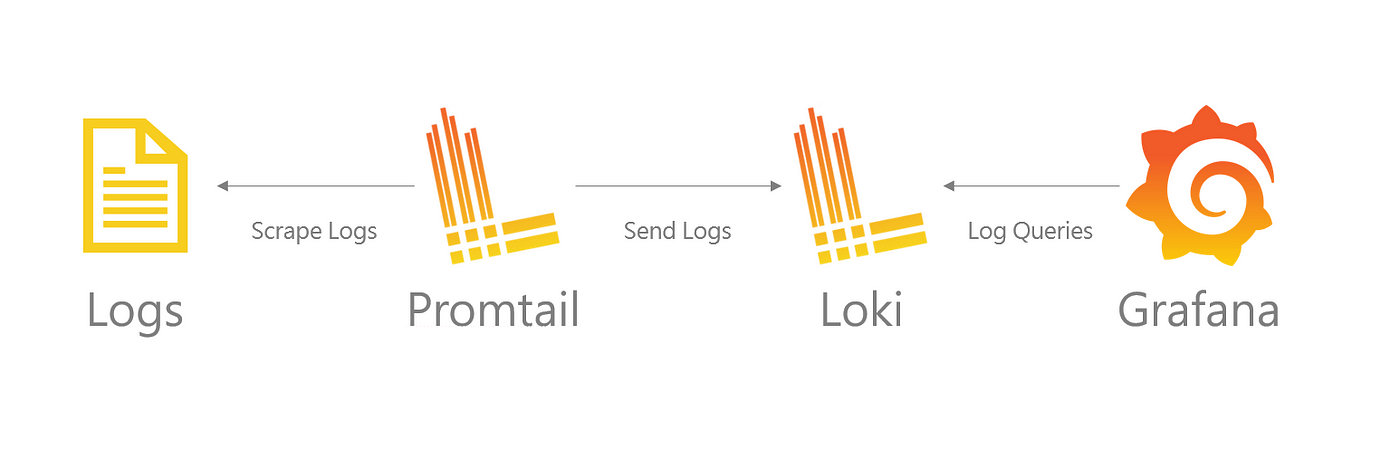
\includegraphics[width=1\textwidth]{./images/loki-promtail.png}
    \caption{Logging architecture.}
    \label{fig:logging_architecture}
\end{figure}

\section{Feature Flag System}
Feature flags are a useful tool for managing software features. They allow system administrators to enable or disable features based on contextual information, such as user roles or location. Feature flags also support A/B testing by enabling controlled rollout, allowing only a subset of users to access a new feature. Additionally, they can be used when integrating a new API into production, allowing testing before deprecating the previous API.

We will not focus on selecting a Feature Flag System. Unleash has provided an objective list of OSS tools that address this need \Parencite{UnleashFeatureFlags}. This is notable, given that Unleash specializes in Feature Flags. It is licensed under the Apache-2.0 license, has 12k stars and 759 forks on GitHub \Parencite{UnleashRepo}, and has been ranked as the top Feature Management Software on G2 \Parencite{UnleashFeatureFlags}. Based on this, we will examine the main features of Unleash rather than other tools. While Unleash offers a more feature-rich enterprise version, the OSS features are sufficient for this project.

\subsection{The Anatomy of Unleash}
Unleash manages feature flags using a client-server architecture. The server controls the feature flags, while the client retrieves and evaluates them via a REST API. The exported endpoints are typically wrapped by a client library, such as the unleash-client-go library for Go, developed by Unleash \Parencite{unleash_client_go_v3}.

Feature flags are organized within projects, which can be used to group related feature flags, teams, or modules. A project can also be assigned per tenant to simulate multi-tenancy. The OSS version supports one project, the Pro version allows up to three, and the Enterprise version supports up to 500 \Parencite{unleash_resource_limits}.

Projects contain environments. The OSS version permits two environments \Parencite{unleash_resource_limits}, which is sufficient for a production environment and an optional development environment if the environments differ. A feature flag is then assigned to an environment. 

\subsection{Activation Strategies}
An activation strategy defines which users receive a feature. It is assigned to a feature flag within an environment. A feature flag can have multiple activation strategies, each evaluated independently. A collection of such reusable activation strategies is called a segment \Parencite{unleash_activation_strategies}.

The default activation strategy is a 100\% gradual rollout, adjustable by setting rollout percentage, targeting, and variants. The rollout percentage determines how many users receive the feature. Targeting specifies which users should be affected, using constraints defined by a context field, an operator, and a value. This allows filtering based on any context. Variants extend a feature flag's payload with additional data to create different versions \Parencite{unleash_activation_strategies}.

\section{Static Website}
Web development involves various technologies and frameworks. Some websites, such as blogs or online CVs, only need to display informational content. In these cases, the Model-View-Controller (MVC) pattern may not be necessary. Instead, static site generators can be used to create static websites. These tools convert plain text files into static HTML pages and are commonly used for blogs, documentation, and content-driven sites.

\subsection{Static Site Generators}
Several static site generators are available, including Jekyll \Parencite{jekyll}, Astro \parencite{astro}, and Hugo \Parencite{hugo}. Each provides templates that allow users to customize their website's appearance. A popular Jekyll theme, Just the Docs \Parencite{just-the-docs}, converts Markdown files into well-formatted HTML pages for online use, making web development more accessible. Documentation should be easy to write; otherwise, it is less likely to be created.

Jekyll, written in Ruby, powers GitHub Pages \Parencite{GitHubPagesJekyll} and organizes content using a simple directory structure. Key folders include \texttt{assets}, \texttt{\_layouts} (for templates), \texttt{\_includes} (for reusable components), \texttt{\_sass} (for styling) and the configuration file \texttt{\_config.yml}. The complete directory structure is available on Jekyll's homepage \Parencite{jekyll}. Content is typically written in Markdown and converted to HTML during the build process. HTML can be directly hardcoded into layouts. The final website consists of static files placed in the \texttt{\_site} folder, which a web server can serve.

\subsection{Web Servers}
Web servers are the backbone of the internet -- they handle requests from users and deliver content like websites, images, and other resources. 

GitHub Pages is a free service to host a static website. It is a great option for hosting documentation, as it is easy to set up and integrates well with GitHub repositories -- it is not even necessary to create a pipeline to deploy the website, as everything is handled by GitHub after enabling the feature. GitHub pages allow one site per repository \Parencite{GitHubPagesLimits}.

NGINX is an HTTP(S) server, reverse proxy, content cache, load balancer, TCP/UDP proxy server, and mail proxy server, distributed under the 2-clause BSD License. It is widely used due to its performance and resource efficiency, making it one of the most deployed web servers and a frequently used Docker image. NGINX also supports multiple Kubernetes Ingress Controllers, including its own \Parencite{NginxWebsite}. 

Using Docker's multi-stage builds, a static website can be created using a single Dockerfile. Earlier stages contain the necessary build tools, while the final image only includes the static files and configuration. This approach optimizes the final Docker image by excluding unnecessary build dependencies, leaving only the NGINX application, its configuration file, and the static HTML files.

\section{Private Registry}
A private registry is used to store and manage container images, allowing organizations to host their own images, control access, and track versions. While Docker Hub is a public registry, it also provides private repositories. GitLab and GitHub offer similar repository services. In some cases, hosting a private registry locally is preferable to prevent images from being pushed outside the firewall. This approach can reduce costs associated with hosted registries or ensure images remain airgapped.

Docker Hub introduced new rate limits, setting a maximum of 10 pulls per hour for unauthenticated users and 100 pulls per hour for authenticated users. This was a significant reduction from the previous limits of 200 pulls per six hours for unauthenticated users and 200 pulls per six hours for authenticated users. In response to user feedback, Docker revisited its policies and decided to maintain the current rate limits \Parencite{DockerHubPolicies}.

To address the limitations, that was later called off, local registries can be implemented as pull-through caches for Docker. Two methods for achieving this are using mirrors \Parencite{dockerhubmirror} or a more advanced solution with Harbor \Parencite{harbor}. This makes Docker pull all images from the local private registry, which in turn pulls the images from Docker Hub if unavailable in the pull-through cache.

\subsection{Mirror}
Mirrors are natively supported in Docker but cannot mirror private registries -- only the central Hub can be mirrored \Parencite{dockerhubmirror}. Configuration consists of two steps.

To set up a registry as a pull-through cache, a proxy section must be added to the configuration file. Parameters include \texttt{remoteurl}, \texttt{username}, and \texttt{password}. The \texttt{remoteurl} specifies the URL of the remote registry to mirror, while \texttt{username} and \texttt{password} provide authentication credentials \Parencite{dockerhubmirror}.

To configure the Docker daemon to use a registry mirror, either pass the \texttt{--registry-mirror} option when starting dockerd, or modify \texttt{/etc/docker/\allowbreak daemon.json} to include the registry-mirrors key \Parencite{dockerhubmirror}.

\subsection{Harbor}
Harbor serves a similar function to a mirror while offering additional capabilities. It is a cloud-native registry that stores, signs, and analyzes content. As an open-source project under the Cloud Native Computing Foundation (CNCF), it is licensed under the Apache License 2.0. Harbor includes a web interface for image management, user authentication, and role-based access control (RBAC). It supports security assessments and integrates with CI/CD pipelines \Parencite{harbor}.

Docker must be configured to use the pull-through cache as described above. In Harbor, proxy settings are established by creating a proxy cache project that connects to a target registry via a registry endpoint \Parencite{harbor}.

\section{Containers \& Virtual Machines} \label{sec:vm_vs_container}
Modern infrastructure relies on technologies that package applications and dependencies while keeping them isolated from the system they run on. Containers provide lightweight environments managed by Kubernetes. KubeVirt extends Kubernetes to support virtual machines, allowing traditional workloads to run alongside containers. NixOS offers a reproducible way to build disk images and manage system configurations.

Virtualization allows a single physical resource, such as RAM, CPU, disk, or networking, to be divided into multiple virtual instances. The main difference between them is that virtual machines simulate an entire system, including hardware, while containers virtualize only the software environment above the operating system \Parencite{atlassian_containers_vs_vms}.

\subsection{Containers}
Containers are lightweight software packages that bundle all necessary dependencies to run an application, including system libraries, third-party code, and other operating system components. They allow quick modifications and iteration, with most container runtime systems providing public repositories of pre-configured containers. These repositories offer access to widely used applications like databases and messaging systems, reducing setup time and simplifying deployment \Parencite{atlassian_containers_vs_vms}.

Shared host exploits may occur because containers share the same underlying hardware below the operating system layer. A vulnerability in one container could allow unauthorized access to the host system, affecting other containers running on the same infrastructure. Public repositories of pre-built containers also introduce risks, as images may contain exploits or be compromised \Parencite{atlassian_containers_vs_vms}.

\subsection{Virtual Machines}
Virtual machines are software packages that emulate low-level hardware components such as CPU, disk, and networking devices. They may also include a software stack to operate on the emulated hardware, creating a fully functional computational system snapshot \Parencite{atlassian_containers_vs_vms}.

Virtual machines provide full isolation security, running as standalone systems. This prevents exploits from spreading between virtual machines on a shared host, ensuring that a compromised machine remains contained. They also support interactive development, allowing manual installation of software and the creation of snapshots to preserve specific configurations. These snapshots can be used to restore a virtual machine to a previous state or deploy additional instances with identical setups \Parencite{atlassian_containers_vs_vms}.

Despite these advantages, virtual machines have limitations. Iteration speed is slower since each snapshot represents an entire system, requiring significant time to regenerate and validate modifications. Additionally, storage size cost can be high, as virtual machines often occupy several gigabytes of disk space, potentially leading to storage constraints on the host system \Parencite{atlassian_containers_vs_vms}.

\subsection{KubeVirt}
KubeVirt is an open-source virtualization API extension for Kubernetes, licensed under the Apache License 2.0 \Parencite{kubevirt_license} and maintained as a Cloud Native Computing Foundation (CNCF) project \parencite{kubevirt_cncf}. It enables the management of virtual machines alongside containers by introducing custom resource definitions (CRDs), which extend Kubernetes to support VM workloads using its native tools. This allows users to run both containerized and virtualized applications within the same cluster, creating a unified infrastructure for diverse workloads.

KubeVirt uses a Docker image based on \texttt{scratch}, where the container disk image, QCOW2, is stored in the \texttt{/disk} directory. QCOW2 is recommended as it reduces image size. The image contains only the disk with no additional content \Parencite{kubevirt_disks_volumes}.

KubeVirt consists of three main cluster components: \texttt{virt-api}, \texttt{virt-\allowbreak controller}, and \texttt{virt-operator}. The \texttt{virt-controller} manages the lifecycle of VMs, while the \texttt{virt-operator} ensures that KubeVirt components are correctly deployed and functioning. The \texttt{virt-api} provides a RESTful interface for interacting with KubeVirt and managing VM resources.

Each virtual machine instance (VMI) is associated with a pod that contains \texttt{virt-launcher}, \texttt{libvirtd}, and \texttt{qemu}. However, the VMI itself does not run within the pod \Parencite{kubevirt_architecture}. Instead, it operates directly on the host as its own instance type: \texttt{virtualmachineinstance.kubevirt.io}. The \texttt{virt-\allowbreak launcher} is responsible for spawning the VM on the host.

If hardware virtualization is unavailable, software emulation can be used instead \Parencite{kubevirt_installation}. In this mode, virtualization is handled entirely by software rather than relying on CPU extensions. Software emulation is expectedly less efficient than hardware virtualization.

\subsection{NixOS Disk Images}
NixOS is a declarative operating system that defines system configurations, including installed packages, services, and settings.

It can build Copy-On-Write version 2 (QCOW2) disk images for virtual machines \Parencite{nixos_vm_configuration}. Using a Nix expression, users generate a QCOW2 image with a predefined environment, ensuring consistency and eliminating manual setup \Parencite{nix_language_tutorial}.

NixOS configurations can be tested in virtual machines without installation on physical hardware. Unlike interactive configuration, which lacks documentation, NixOS provides a structured approach. Interactive setups make modifications difficult and do not track changes, leading to uncertainty about the image's contents.

This approach allows image generation at runtime instead of storing large QCOW2 images. Since they cannot be stored in Git due to their size, declarative configuration enables automated, reproducible builds when needed.

\section{Static Code Analysis}
Static code analysis is a software testing technique that examines code without executing it, serving as the counterpart to dynamic code analysis. It is used to identify potential vulnerabilities, bugs and code smells. Static code analysis can be performed manually or automatically using tools. The latter is more efficient and less error-prone, as it can be integrated into the development process.

In this section we will cover the tools used in this project for static code analysis. These tools include Dependabot, SonarCloud, and Linting.

\subsection{Dependabot}
Dependabot is a dependency management tool rather than a static code analysis tool. It is included in discussions of repository scanning because it identifies outdated dependencies, checks for updates, and creates pull requests to keep them current. It also provides security alerts for known vulnerabilities in dependencies, helping developers address risks promptly. Dependabot supports package managers such as pip, npm, and Maven and can be configured to check for updates on a schedule \Parencite{GitHubDependabotVersion2025}.

\subsection{SonarCloud}
SonarCloud is a cloud-based platform for continuous code quality and security inspection. It performs static code analysis to detect bugs, vulnerabilities, and code smells, supporting multiple programming languages. Integrated seamlessly with CI/CD pipelines, it enables automated code quality checks throughout development \Parencite{SonarQubeDocs2025}.

The service offers a web interface for monitoring quality metrics and trends over time. It is free for public repositories; however, private repositories require a paid subscription \Parencite{SonarCloudPricing2025}. In contrast, SonarQube is a self-hosted solution, licensed under the GNU Lesser General Public License v3.0 \Parencite{SonarQubeLicense2025}. It provides similar functionality and supports private repositories -- while the Community Edition is free, advanced plans come at a cost.

\subsection{Linting}
Linting is a static code analysis technique used to detect errors, enforce coding standards, and improve code readability. Some linters assess cyclomatic complexity, helping developers understand the maintainability of their code. By identifying issues early in the development process, linting ensures consistency and enhances code quality. Linting tools can be integrated into IDEs or run as part of the build process \Parencite{SuperLinter2025}. Popular options include ESLint for JavaScript, Pylint for Python, and SonarQube for IDE (formerly SonarLint), which supports multiple programming languages.

SonarQube for IDE integrates automated code review into your development environment \Parencite{SonarQubeConnectedMode2025}. Connected mode links projects to SonarQube Cloud or Server, ensuring consistent best practices, preventing security vulnerabilities, and reducing technical debt before code is committed.

\chapter{Implementation}\label{chap:implementation}
This chapter outlines the implementation of a scalable, secure, and fault-tolerant CTF platform, building on prior concepts and technologies. The MVP is considered complete when the platform supports multiple users who can create, manage, and participate in challenges. Additionally, it must provide documentation for users, administrative monitoring, and robust security measures, including encrypted access and fault tolerance.

\section{Architecture}\label{sec:architecture}
The architecture of the CTF platform is designed to be modular and extensible, allowing for easy integration of new features and services. The platform is built on a microservice architecture, with each service responsible for a specific functionality. This approach enables independent development, deployment, and scaling of services, ensuring that the platform can adapt to changing requirements and user needs.

UCloud was never selected for its capabilities but for its affordability. While the availability of UCloud resources through the university was an advantage, the challenges of building a usable and widely accessible platform remained significant -- though solving them was an engaging task. This section first presents the architecture as it was successfully implemented on UCloud before detailing its final deployment on GCP. Although GCP is an expensive option, it was the only one investigated that provides hardware virtualization, a required capability for the platform.

\subsection{Services}

Figure \ref{fig:architecture} illustrates the UCloud architecture. Network limitations posed a significant challenge, which was mitigated by implementing a Headscale network overlay and integrating a GCP VM. The GCP VM served as the entry point and login server for the Headscale network. All nodes, including GCP itself, are connected through this login server using Tailscale, enabling communication across nodes without the usual network restrictions. Tailscale is a VPN based on WireGuard \Parencite{TailscaleDocs}, while Headscale is a self-hosted alternative to Tailscale's coordination server \Parencite{TailscaleOpenSource}. 

\begin{figure}[h]
    \centering
    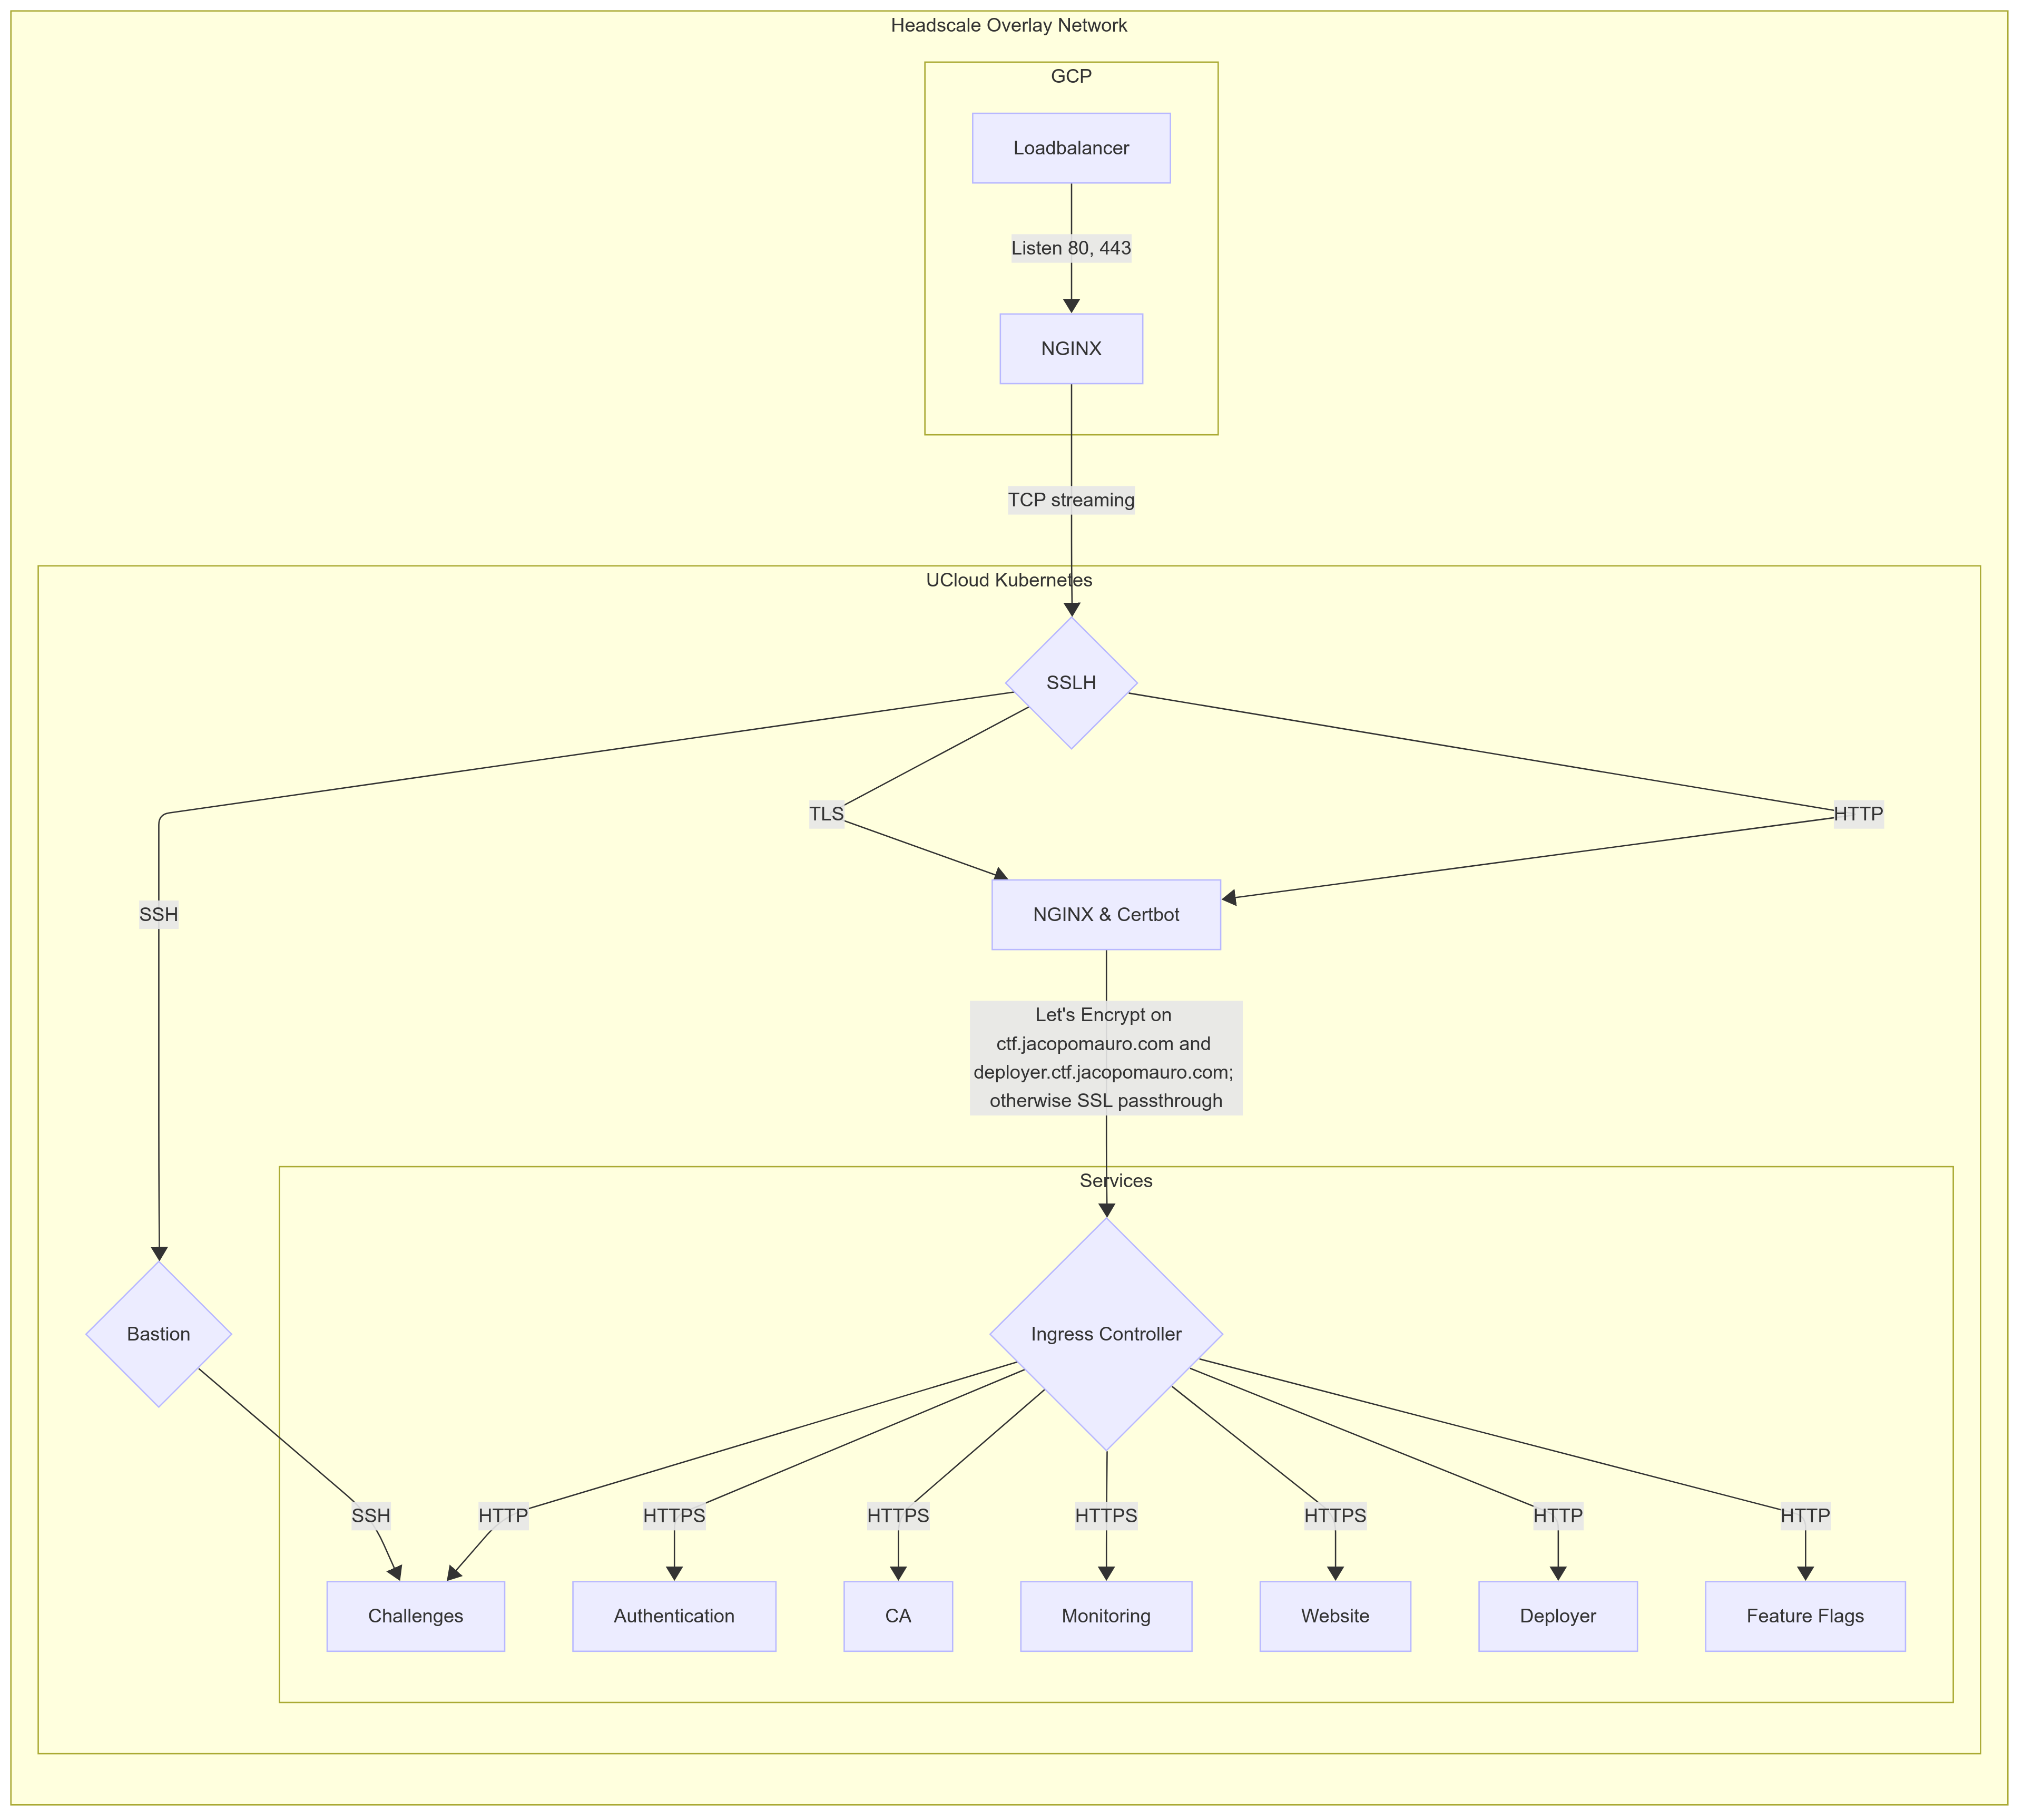
\includegraphics[width=1\textwidth]{images/ucloud-architecture.png}
    \caption{Architecture of the CTF platform deployed on UCloud.}
    \label{fig:architecture}
\end{figure}

The NGINX instance on GCP facilitates TCP streaming to UCloud, as this approach proves optimal for the Bastion. Initially, GCP was only used as a login server, since SDU offered a domain name for free. The domain name had to point to a UCloud VM and was linked to a proxy that applied the certificate and forwarded requests to the UCloud server. While the wildcard certificate was useful, handling TLS termination at the cluster level was preferred.

SSLH is a protocol multiplexer that routes traffic to different services based on the detected protocol. It is used to direct SSH traffic to the Bastion while forwarding HTTP(S) traffic to the NGINX/Certbot proxy. This setup prevents SSH traffic from reaching the proxy, which is unable to handle it, and ensures that no certificates are applied to SSH connections, avoiding the need for users to tunnel SSH via TLS.

The trusted TLS certificate could have been managed at the ingress controller instead of the Certbot proxy. This approach was chosen because it simplifies the setup, allowing all internal services to use certificates issued by our own PKI. Rather than modifying this configuration for production deployment, adding a proxy in front of the system to handle TLS termination makes the adjustment more straightforward.

The remaining architectural details will be covered in their respective sections, as they pertain to platform functionality rather than system architecture. The \textit{services} box in Figure \ref{fig:architecture} represents the core components of the platform, while all other elements ensure secure access to these services for users.

Migrating this architecture to GCP simplifies the setup significantly. In fact, everything outside the UCloud Kubernetes box in Figure \ref{fig:architecture} can be removed. With this change, SSLH serves as the new entry point, eliminating both the network overlay and the additional proxy forward. 

\subsection{Storage}

We recognize that building a completely fail-safe system is unrealistic; instead, our priority is to create a safe-to-fail system. When shit hits the fan, a full redeployment of the platform may be necessary. In such cases, minimizing downtime is crucial, but protecting data integrity is non-negotiable. To eliminate this risk, we have opted for object storage buckets in MinIO, ensuring robust and reliable data management. The setup is illustrated in Figure \ref{fig:storage-provisioning}.

\begin{figure}[h]
    \centering
    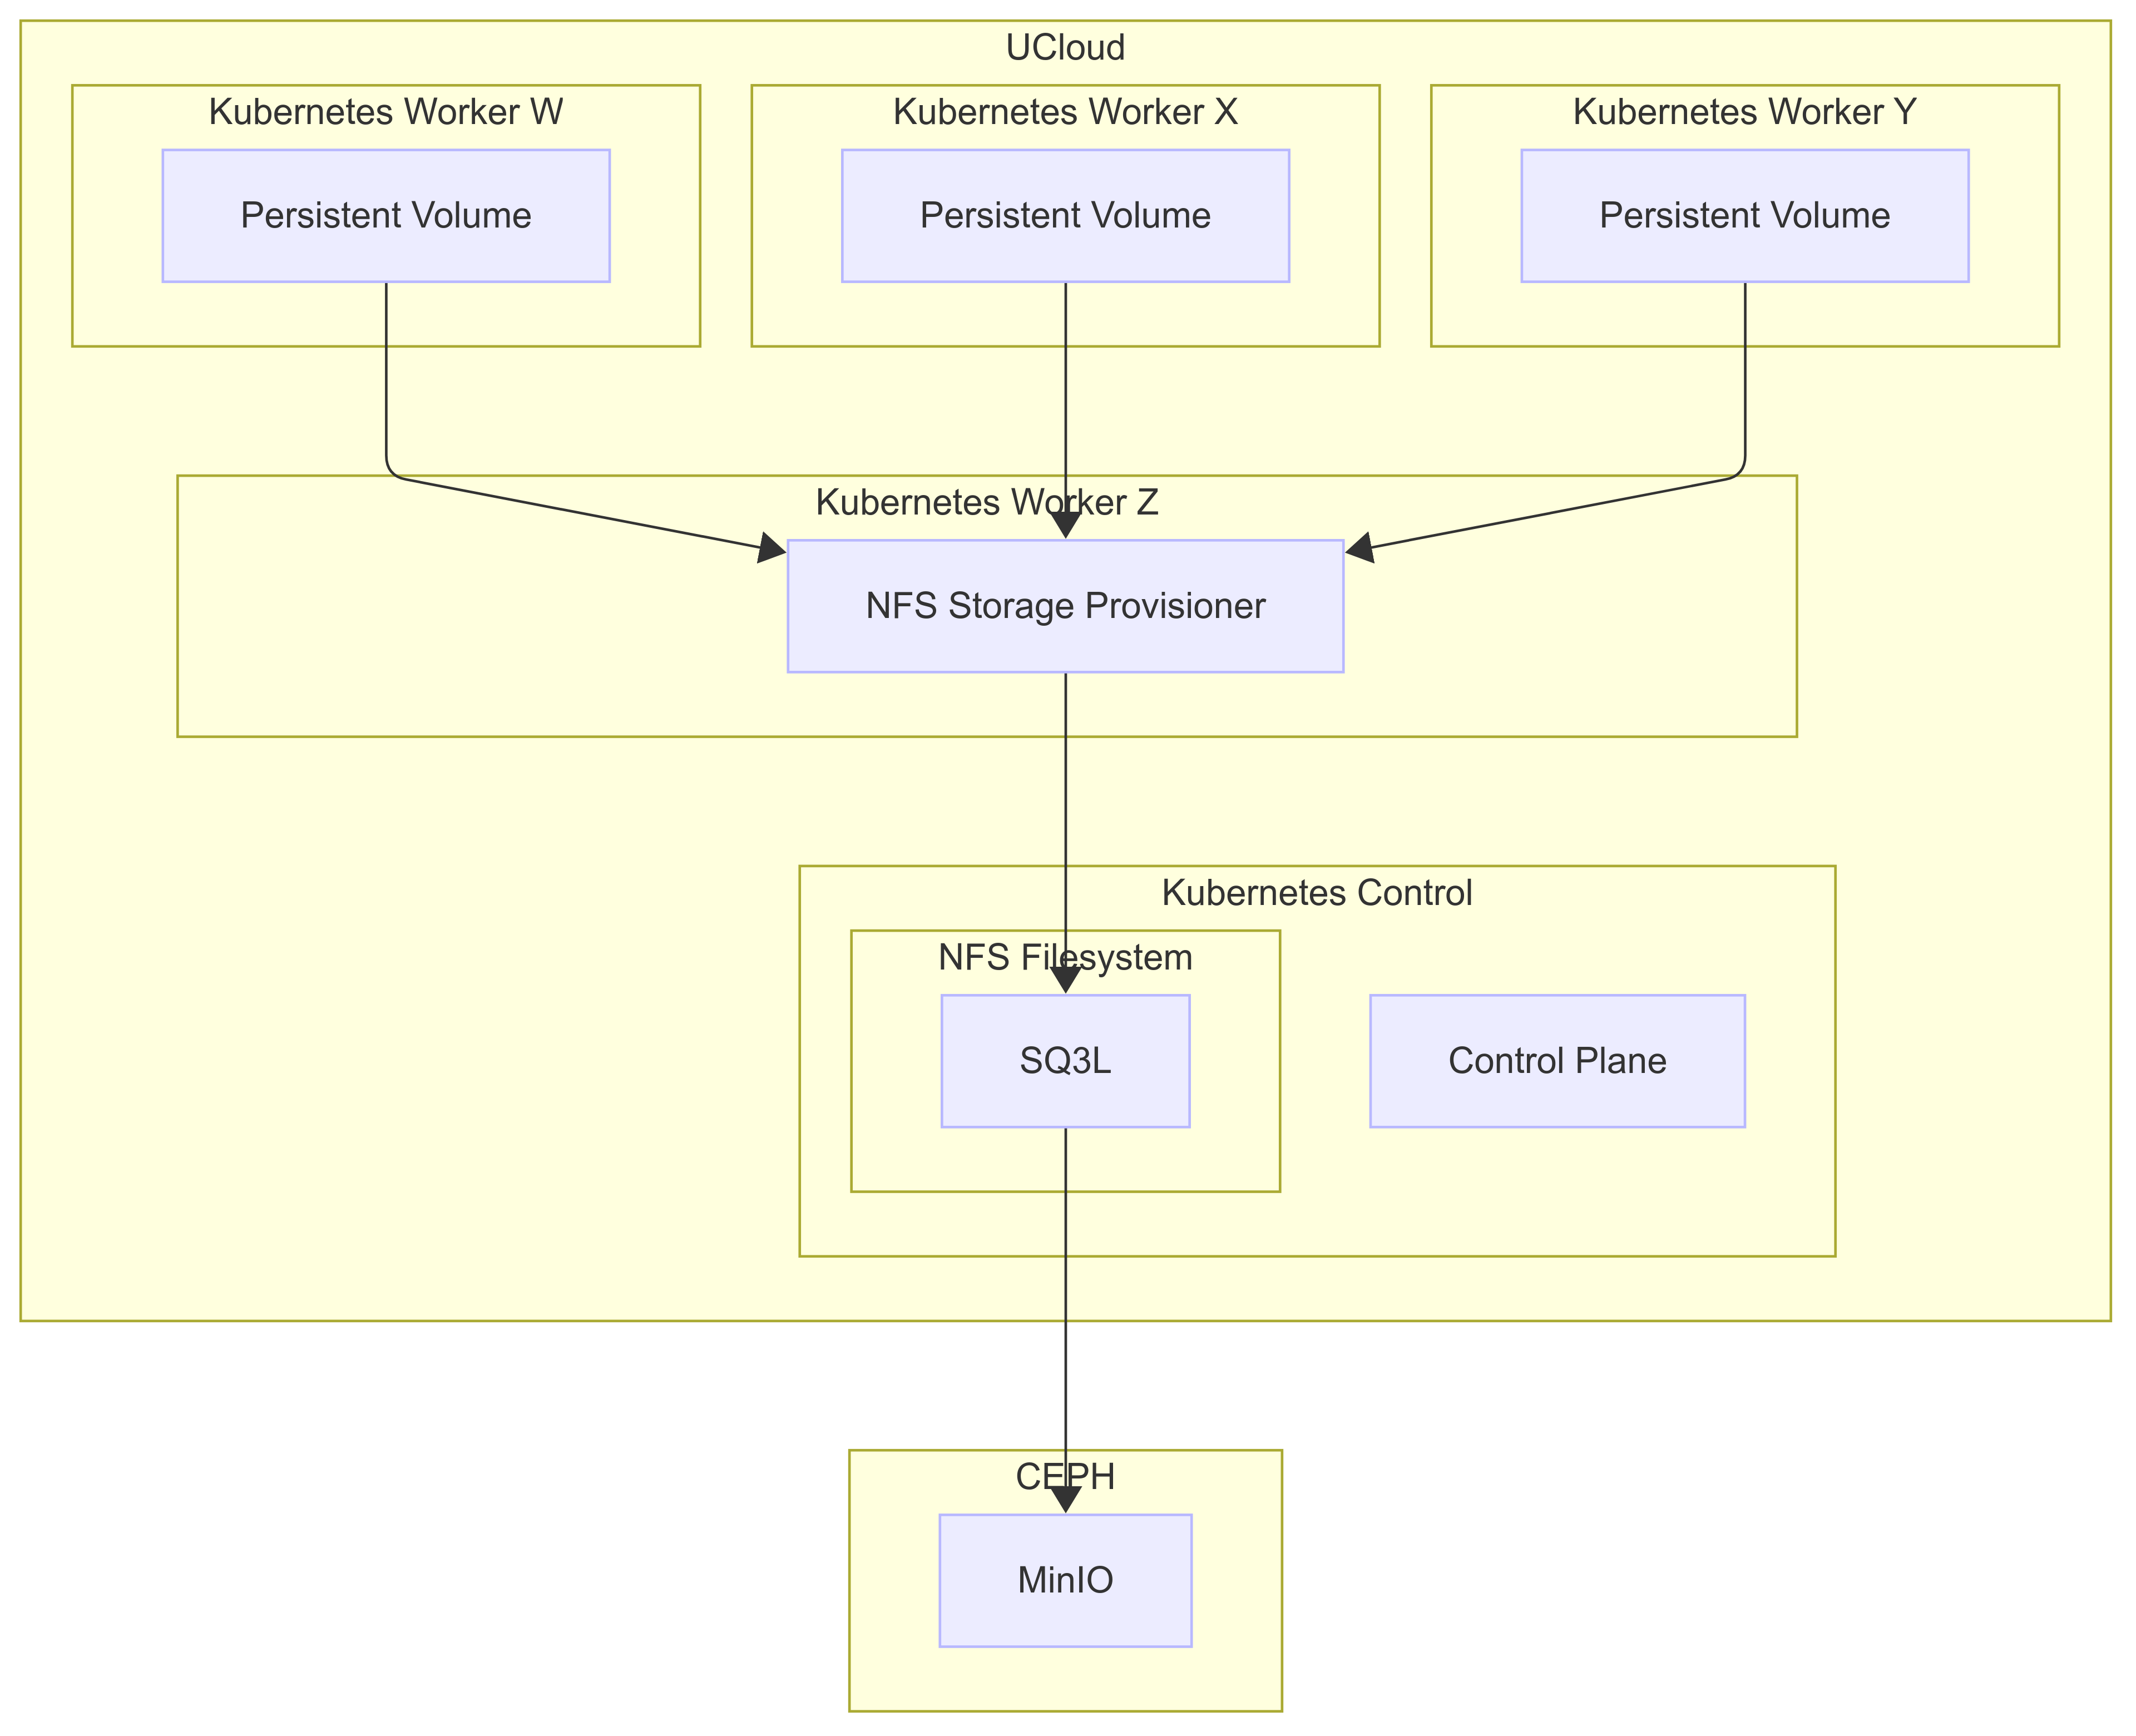
\includegraphics[width=1\textwidth]{images/storage-provisioner.png}
    \caption{Storage provisioning architecture of the CTF platform on UCloud using MinIO.}
    \label{fig:storage-provisioning}
\end{figure}

The architecture initially relied on the Rancher Local Path Provisioner, configured as a shared filesystem using the \texttt{hostPath} volume type to store data on a specified path on the host. As retaining data across VM restarts became a necessity, we introduced MinIO as an object storage solution \Parencite{miniosdu}. To integrate MinIO, we first adopted S3FS, a FUSE-based filesystem, but it lacked support for certain filesystem operations, causing databases to crash when interacting with it \Parencite{s3fsrepo}. To resolve this, we replaced S3FS with S3QL, another FUSE-based filesystem that provides full filesystem functionality \Parencite{s3qlrepo}. However, S3QL could not be mounted on multiple nodes simultaneously \Parencite{s3qlfaq} -- a critical requirement for the current setup. To address this limitation, we transitioned from the Local Path Provisioner to an NFS storage provisioner, consolidating all storage within a single folder on the control node, where S3QL is mounted on the same path as MinIO, allowing MinIO to provide block storage while S3QL handles filesystem operations.

The NFS provisioner provides the same benefits as a shared filesystem: pods are not restricted to the same node as the storage, allowing them to be scheduled on the least-loaded node -- even after restarts.

Migrating this architecture to GCP introduces minimal changes. Instead of using MinIO, we leverage GCP's persistent disks for storage, while the rest of the architecture remains unchanged.

\section{Pulumi}
Pulumi's ability to use Terraform providers makes it well-suited for managing the entire infrastructure. However, Terraform was introduced in this project primarily due to existing expertise within the team. The author of this thesis works with Pulumi, while Matteo Trentin manages Terraform -- this division is based on individual proficiency. While the goal is to maintain a simple technology stack, compromises are necessary in a team environment with tight deadlines. If needed, this setup can be adjusted in the future. This thesis focuses on Pulumi, as the Terraform IaC was not developed by the author.

\subsection{Projects \& Stacks}
When starting a new project, it is essential to determine how to organize the Pulumi project and its stacks. To assist in this decision, the Pulumi documentation provides insights into the trade-offs between different approaches \Parencite{pulumiProjects2025}.

The monolithic approach is well-suited for projects that prioritize simplicity, version control, and agility. This method makes it easier to track dependencies, configure package managers, and manage code efficiently, as everything can be previewed and handled in a unified manner.

The micro-stacks approach, similar to microservices but applied to projects and stacks, offers greater independence. Each stack can be deployed separately, making it ideal for projects with varying deployment cadences. Security is another key factor. Large organizations often require Role-Based Access Control (RBAC), which makes micro-stacks advantageous. This approach enables fine-grained access control, ensuring that critical infrastructure can only be modified by selected team members.

For this project, a hybrid approach was adopted. While it primarily relies on micro-stacks, keeping related components together, it also incorporates monolithic elements since the stacks are not entirely independent. The stack organization follows a layered structure. The base layer includes essential components like Custom Resource Definitions (CRDs), secret generation, storage provisioner, KubeVirt, namespaces, and the ingress controller. Directly above this is the PKI, responsible for certificate issuance. 

The remaining stacks exist on the same hierarchical level. The Monitoring stack is completely independent, collecting metrics and logs from the Kubernetes cluster in a passive, non-intrusive manner. Monolithic traits arise in the Application stack, as it combines various unrelated services. While the authentication stack is independent, certificates depend on it for issuing personal SSH certificates, creating a circular dependency (explained in Section \ref{sec:smallstep}).

High coherence and low coupling are vital for effective stack design. While it is important to group only related elements together, the decision to create new stacks should align with the project's scope and complexity. For smaller projects, maintaining simplicity is often more practical. The stack relationships are visually represented in Figure \ref{fig:pulumi_stacks}.

\begin{figure}[h]
    \centering
    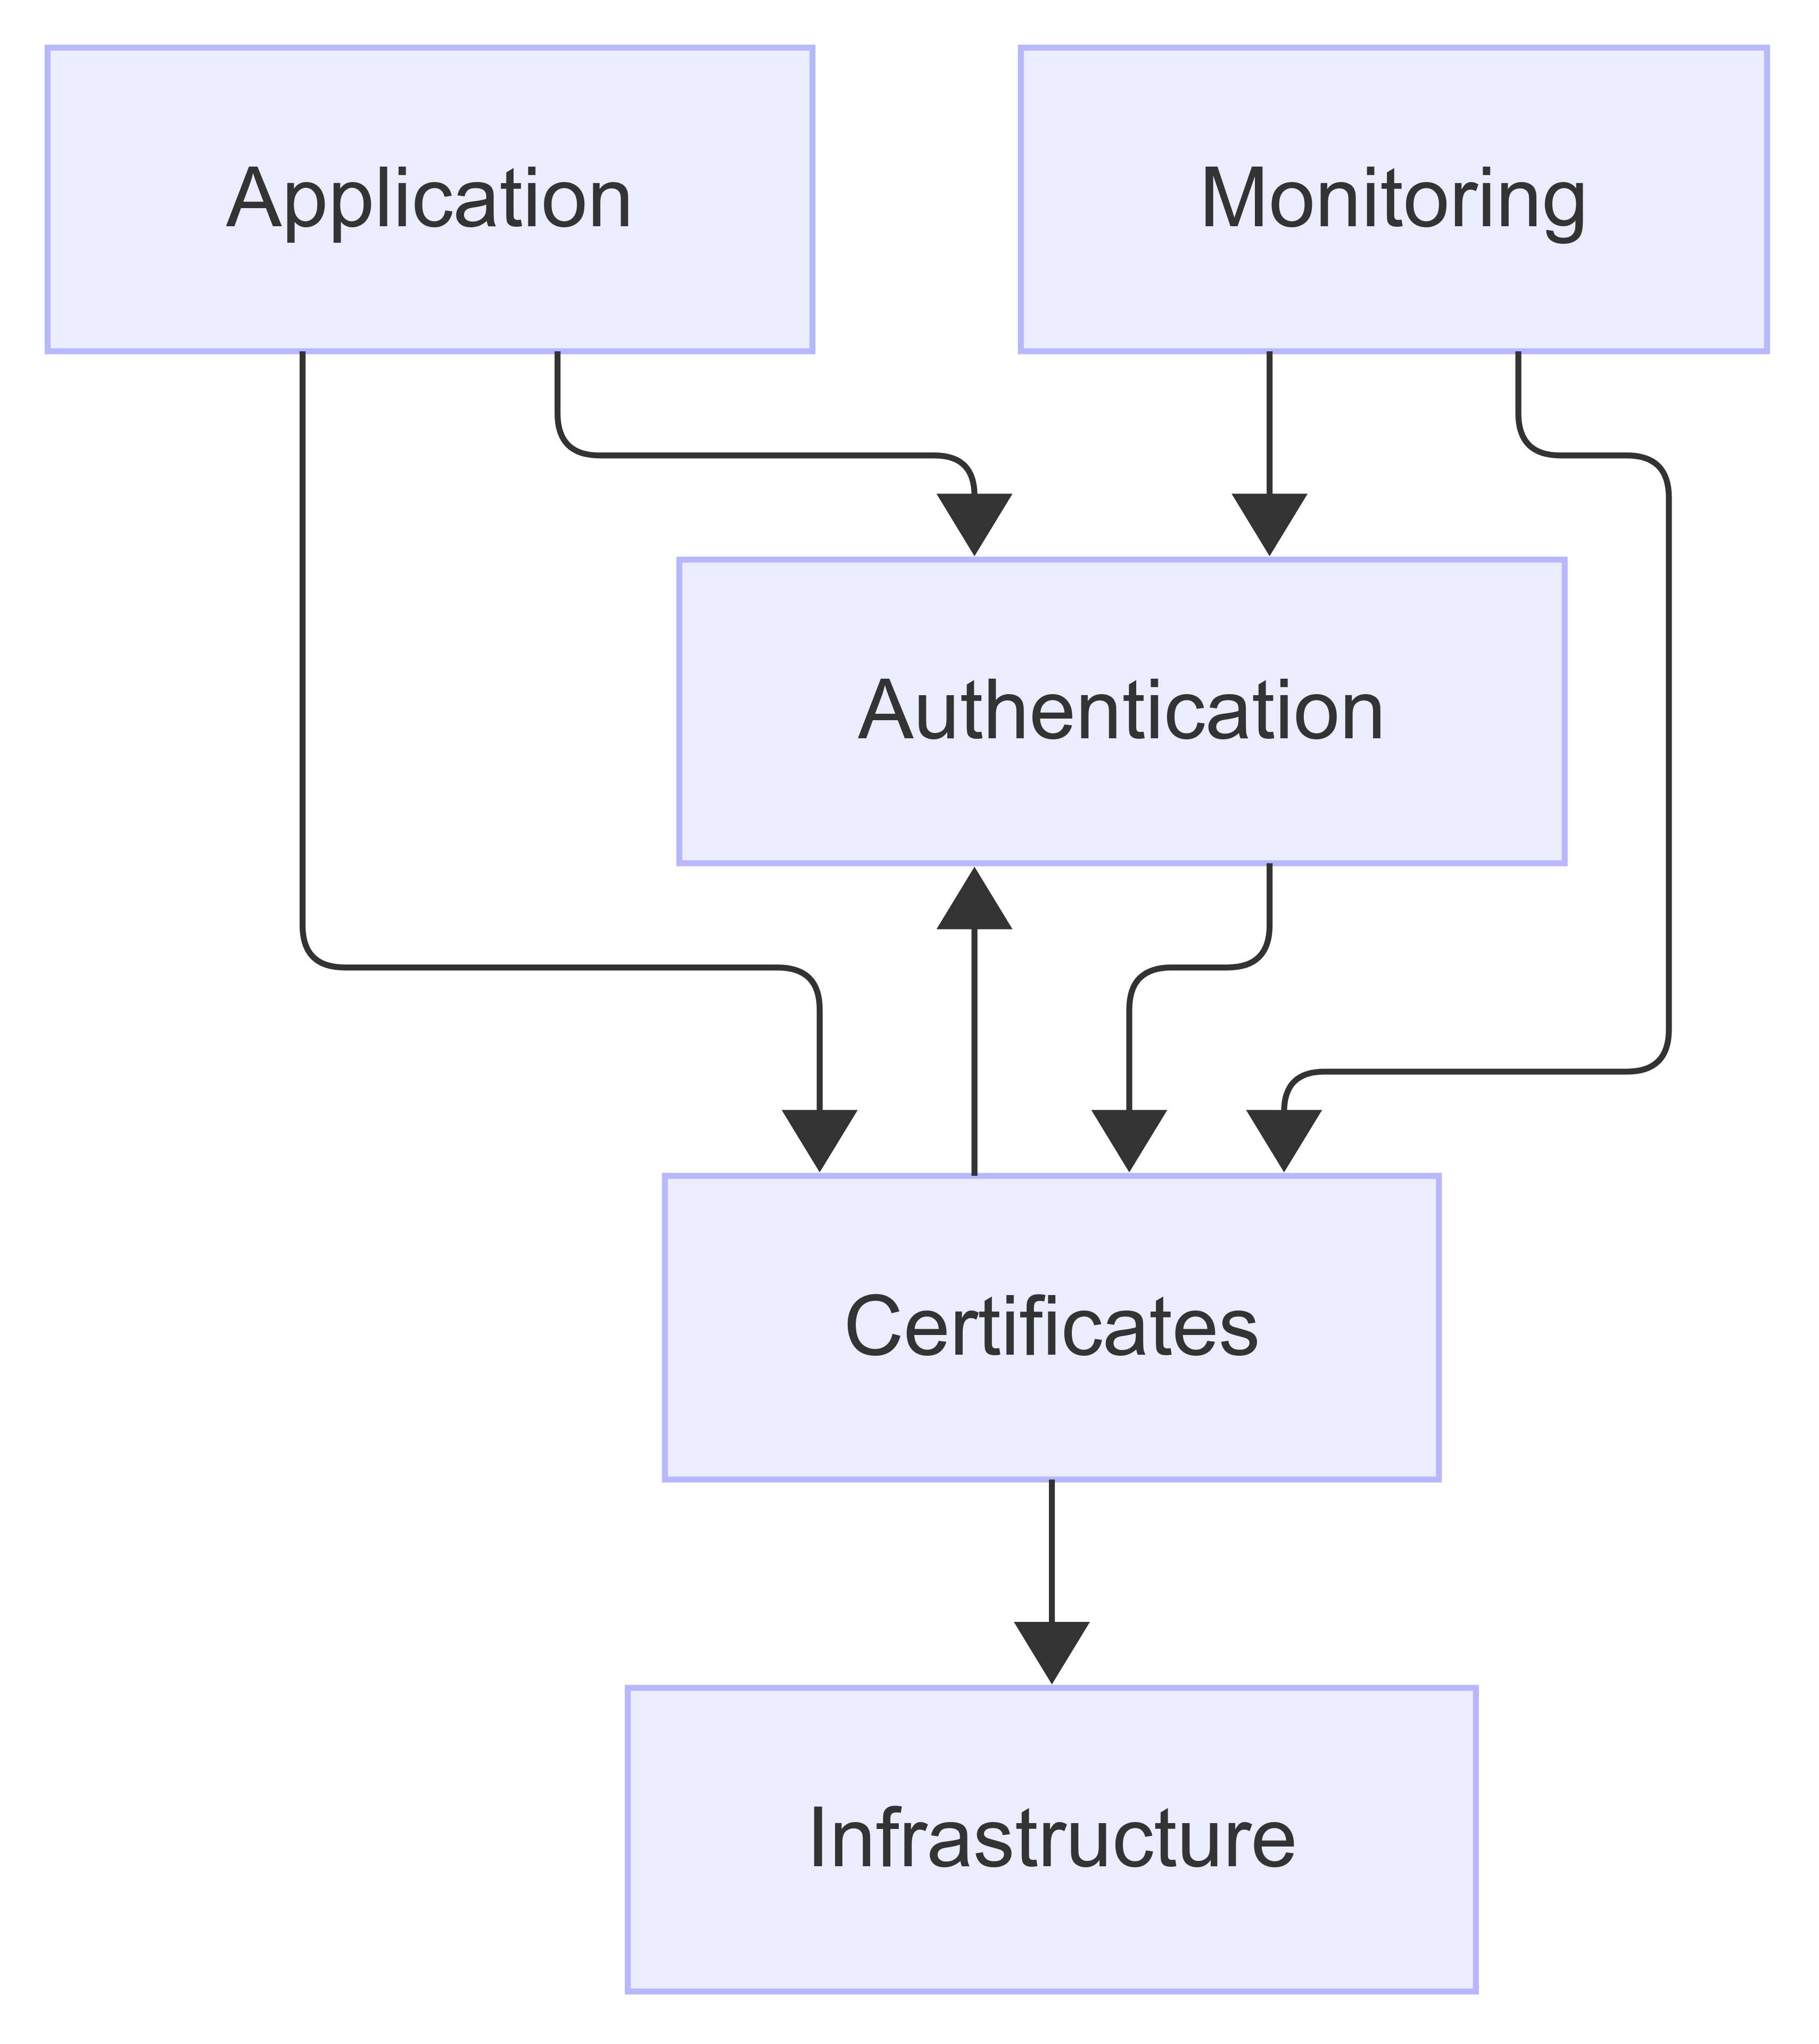
\includegraphics[width=.5\textwidth]{images/pulumi_stacks.png}
    \caption{Pulumi Stacks Relationship. An arrow pointing from a source to a target indicates that the source depends on the target. Given the layered approach, these relationships are transitive. However, arrows targeting certificates are explicitly included due to their significance.}
    \label{fig:pulumi_stacks}
\end{figure}

Our project consists of five Pulumi projects, each with a specific role to play:

\begin{itemize}
    \item \textbf{Application:} Home to CTF platform/cloud-specific functionality.
    \begin{itemize}
        \item \textbf{Homepage:} A user guide for navigating and utilizing the platform.
        \item \textbf{SSHD Alpine bastion:} A secure SSHD server based on Alpine Linux, serving as a bastion host for your cloud environment.
        \item \textbf{CTFd:} A CTF platform for hosting cybersecurity challenges and competitions.
        \item \textbf{Deployer Backend:} The backend service providing core functionality and APIs for the platform.
        \item \textbf{SSLH protocol multiplexer:} A protocol multiplexer that allows multiple services to share a single port, such as SSH and HTTPS.
        \item \textbf{NGINX Proxies:} Proxies to upgrade connection and/or move SSL termination to pod.
        \item \textbf{Unleash:} An open-source solution for feature flagging.
        \item \textbf{Reflector:} A Kubernetes utility that automatically mirror secrets across namespaces.
        \item \textbf{Docker Registry:} A system for storing and sharing Docker images.
    \end{itemize}
    \item \textbf{Monitoring:} Ensures cluster observability and log collection.
    \begin{itemize}
        \item \textbf{Prometheus:} A monitoring system and time-series database for capturing metrics and alerts.
        \item \textbf{Prometheus-Operator:} Simplifies the setup and management of Prometheus instances within Kubernetes.
        \item \textbf{Grafana:} An open-source platform for monitoring and observability, providing dashboards and visualizations for your metrics.
        \item \textbf{Loki:} A log aggregation system designed for efficiency and ease of use, seamlessly integrating with Prometheus.
        \item \textbf{Promtail:} An agent that ships the contents of local logs to a Loki instance.
        \item \textbf{Node-exporter:} Exports hardware and OS metrics exposed by Linux kernels for monitoring.
    \end{itemize}
    \item \textbf{Authentication:} Manages SSO capabilities provided by Keycloak.
    \begin{itemize}
        \item \textbf{Keycloak:} An open-source identity and access management solution for SSO, enabling secure authentication and authorization.
    \end{itemize}
    \item \textbf{Certificates:} Handles certificate CA and issuers.
    \begin{itemize}
        \item \textbf{Step Certificates:} A CA toolkit for managing and issuing certificates within your environment.
        \item \textbf{Step Autocert:} Automates the issuance and renewal of TLS certificates to ensure your services remain secure.
        \item \textbf{Step Issuer:} An issuer that integrates with Cert-Manager to manage certificate lifecycles.
        \item \textbf{Cert-Manager:} A Kubernetes add-on to automate the management and issuance of TLS certificates from various issuing sources.
    \end{itemize}
    \item \textbf{Infrastructure:} Takes care of basic cluster configuration.
    \begin{itemize}
        \item \textbf{NFS Storage Provisioner:} Manages dynamic storage provisioning for Kubernetes using NFS, enabling shared storage across nodes.
        \item \textbf{Nginx Ingress Controller:} Manages external access to services in a Kubernetes cluster through HTTP and HTTPS.
        \item \textbf{KubeVirt:} Extends Kubernetes by adding support for running virtual machine workloads alongside container workloads.
    \end{itemize}
\end{itemize}

These are the core services of the platform. Some provide direct user-facing functionality, while others support essential technical operations. Additionally, the platform includes sidecar containers, which are not listed here.

\subsection{Managing Secrets}
Pulumi includes a built-in mechanism for managing secrets. The user provides a passphrase, which is combined with the encryption salt stored in each stack to encrypt secrets. However, these stacks can also include configuration values in plain text. Secrets can be added using the following command:

\begin{minted}{bash}
    pulumi config set --stack <stack> --secret <key> <value>
\end{minted}

And configuration values can be added using the following command:

\begin{minted}{bash}
    pulumi config set --stack <stack> <key> <value>
\end{minted}

This mechanism functions similarly to a password vault, where all secrets are safeguarded by a single master passphrase. As such, it is crucial to ensure that this passphrase is never compromised. While passwords within the stack can be rotated, the passphrase represents a single point of failure.

In case the passphrase have been compromised, it can be updated using the command:

\begin{minted}{bash}
    pulumi stack change-secrets-provider passphrase --stack <stack>
\end{minted}

Only passwords that must be explicitly known, such as Keycloak login credentials, are stored within the stacks. Passwords that only need to be used by the system are generated during deployment. For example, knowing the database password provides no benefit since it is solely used by the application. Similarly, client credentials for OAuth2 clients are designed to remain confidential. By ensuring that these passwords are not accessible, the risk of them being leaked is eliminated, at least to some extent -- any application can be compromised from within.

Generating secrets during deployment ensures fresh credentials with each update but introduces challenges in password rotation. The current implementation generates most passwords at deployment, simplifying initial setup but causing issues for components that rely on persistent credentials, particularly databases that retain old passwords tied to user accounts. If passwords are sourced from the state file, stack updates would not generate new credentials, preventing automatic password rotation. Conversely, enabling password rotation requires migration steps to avoid authentication failures. This suggests that dynamically generating secrets may not always be ideal. Hardcoding secrets directly in the Pulumi stack offers a predictable and controlled approach but increases the risk of exposure. Choosing between these methods requires careful consideration of security, operational needs, and long-term maintainability.

In a monolithic stack, all information is already available within the same stack. When using a micro-stack architecture, it may be necessary to share information between stacks. Stack references make this possible by allowing one stack to access outputs from another, such as randomly generated secrets, or other stack-specific data. This enables generating all secrets in the Infrastructure stack and exporting them to the services that need them.

\subsection{Helm Charts}
Pulumi offers two approaches for deploying Helm charts: as a \texttt{Chart} \Parencite{PulumiHelmChart} or a \texttt{Release} \Parencite{PulumiHelmRelease}. The key difference lies in how Pulumi manages these resources. When using \texttt{Chart}, Pulumi treats all resources within the chart as its own, incorporating them into its state. Conversely, the \texttt{Release} option deploys the Helm chart as a release, meaning the resources are not tracked in Pulumi's state and are managed independently. This approach is useful for charts intended to be managed outside of Pulumi or when keeping the Helm release separate from a Pulumi stack.

One important consideration is that Helm hooks are no longer supported in Pulumi Charts v4. While Chart v3 also lacked hook support, it historically emitted hooks as ordinary child resources. Another notable improvement in Chart v4 is enhanced resource ordering \Parencite{PulumiKubernetesChartV4}. For example, in Chart v3, deploying \texttt{kube-prometheus-stack} was problematic because services dependent on CRDs were created before the CRDs themselves were available. This required manually installing the CRDs within the Infrastructure stack. Chart v4 eliminates this workaround by handling resource ordering automatically. However, the CRDs remain in the Infrastructure stack for flexibility, ensuring availability for other stacks beyond Monitoring -- \texttt{ServiceMonitors}, for example, are widely used across different stacks.

Why use Helm charts at all? The primary advantage is their active community maintenance, which ensures regular updates and improvements. Helm charts bundle numerous resources, reducing the complexity of manually defining and managing them. They provide a streamlined, efficient way to configure and deploy applications compared to writing everything from scratch. Given these benefits, we will rely on Helm charts in this project whenever possible.

In conclusion, Helm charts are preferred over manual resource definitions, and Pulumi Charts v4 will be used to manage their deployment.

\section{Ansible}
Terraform is used to provision the servers. However, since UCloud does not provide a Terraform provider, an alternative approach was required for deploying Kubernetes resources. To address this, we leveraged Ansible -- an agentless automation tool that uses SSH to connect to servers and execute commands remotely, eliminating the need for software installation on target machines.

The majority of the Ansible work has been completed by Matteo Trentin, though I have contributed to specific aspects outlined in this section. My primary contributions include deploying Pulumi stacks, configuring the NFS server, making sure that \texttt{Kubectl} used the Tailscale subnet\footnote{Only needed when deployed on UCloud.}, and developing a deep understanding of the existing Ansible playbooks and roles.

\subsection{Playbook}
The playbook is a core component of Ansible, defining the automation workflow. It is a YAML file that specifies the target hosts, assigned roles, and the tasks to be executed. The playbook follows a structured process: First, common tools are installed on all nodes, including both control and worker nodes. Next, the control node is configured -- setting up the Kubernetes control plane, mounting MinIO, and starting the NFS server. Then, the worker nodes are configured and joined to the Kubernetes cluster. Finally, the Pulumi stacks are deployed on the control node.

The target hosts are specified in the \texttt{hosts.ini} file located in the \texttt{ucloud-k8s/\allowbreak ansible} folder. This file contains the IP addresses of the nodes, enabling SSH connections for task execution. The playbook is executed using the \texttt{ansible-playbook} command, which processes the YAML file and runs the defined tasks on the target hosts. Additionally, the host file includes variables required by various tasks. Since \texttt{hosts.ini} contains environment-specific details, it is not stored in version control. Instead, a template file, \texttt{hosts.ini.example}, is provided as a reference.

\subsection{Deployment}

Before executing the playbook, it is essential to configure the \texttt{hosts.ini} file and set up the required secrets.

The \texttt{hosts.ini} file in the \texttt{ansible} directory defines the inventory of hosts managed by Ansible -- use the \texttt{hosts.ini.example} template to create it.

A few secrets are required for secure access and configuration management. An SSH key pair must be generated and stored in the location specified in \texttt{ansible/ansible.cfg} for server access. A \texttt{pulumi\_passphrase} file should be placed at the repository root to manage Pulumi stack encryption. If deploying on UCloud, a Tailscale authentication key must be stored in \texttt{tailscale\_key} at the repository root for machine authentication, with its location adjustable in the ``connect to Tailscale'' task within the Tailscale role.

A rigorous and continuously updated deployment guide is available online at \url{https://kianbankelarsen.github.io/CTF-Platform/ucloud-k8s/}. As the codebase evolves, this guide provides the latest instructions to ensure a seamless deployment process.

\section{CTFd Plugins}
CTFd is a web-based platform designed to host CTF competitions \Parencite{ctfd_github}. It is built using Flask, a Python web framework, and provides a user-friendly interface for managing challenges, teams, and scoring. CTFd is open-source, distributed under Apache License 2.0 \Parencite{ctfd_github}, and can be self-hosted using a Docker image \Parencite{ctfd_docker}. The platform is designed to be extensible, allowing developers to create custom plugins to enhance its functionality. This extensibility is a key feature of CTFd, enabling users to tailor the platform to their specific needs and requirements. 

This section provides insight to the CTFd plugins developed for the platform. The first plugin is a custom authentication plugin that integrates with Keycloak, enabling SSO capabilities. The second plugin is a custom challenge plugin that allows users to start a challenge managed by our Deployer Backend. 

\subsection{Authentication}

CTFd requires an authentication system to manage user access. Instead of handling user creation internally, external identity providers can be integrated to streamline authentication. While Keycloak is not configured to use an external Active Directory, it enables SSO, allowing participants to authenticate using accounts created within Keycloak.

Despite this integration, CTFd does not natively support SSO unless using an enterprise or hosted version \parencite{ctfd_sso}. This limitation presents a challenge and requires a decision on how to proceed. Given that CTFd is open-source, we have two options: modify the source code to implement SSO directly or develop a custom plugin for authentication. Modifying the core code would require freezing the version. Therefore, creating a plugin is the more practical and maintainable approach. Fortunately, creating plugins for CTFd is relatively straightforward and well-documented \parencite{ctfd_plugins}. 

The plugin is configured via \texttt{config.json}, which is loaded at initialization to define its behavior using basic OIDC parameters. A decision is required for handling the client secret -- either embedding it in the configuration file or providing it as an environment variable. Storing it in the configuration file would bake it into the image, which is undesirable, while using an environment variable keeps it separate but leaves the configuration file incomplete. Since Pulumi generates the secret dynamically, it cannot be set statically in the configuration. Instead, \texttt{OIDC\_CLIENT\_SECRET} is defined as an environment variable, replaced at runtime. Pulumi loads the config, performs environment substitution, and mounts the updated file in the appropriate location. Additionally, the config file supports specifying the path to a certificate bundle when the connection to the identity provider must be manually trusted.

Overwriting authentication endpoints allows us to redirect authentication flows to our implementation instead of relying on CTFd's default mechanisms. This facilitates integration with Keycloak, ensuring all login and logout operations are managed through our identity provider. Additionally, modifying these endpoints enables control over user management actions, such as disabling registration and password resets. However, disabling the registration endpoint does not remove the registration button, so registration must be set to private during the initial setup wizard of CTFd.

\begin{minted}{py3}
app.view_functions['auth.login'] = lambda: redirect(url_for('keycloak'))
app.view_functions['auth.logout'] = lambda: redirect(url_for('keycloak_logout'))
app.view_functions['auth.register'] = lambda: ('', 204)
app.view_functions['auth.reset_password'] = lambda: ('', 204)
app.view_functions['auth.confirm'] = lambda: ('', 204)
\end{minted}

The implementation uses \texttt{python-keycloak} \parencite{python_keycloak}, a client tool designed for handling authentication with Keycloak. While a more general approach could have involved using a generic OIDC plugin, \texttt{python-keycloak} was chosen for its ease of use and effectiveness in addressing our specific needs. 

The OIDC plugin is configured to follow the authorization code flow as recommended by the Keycloak documentation. The authentication process operates as follows:

\begin{enumerate}
    \item A user logs into CTFd using their SSO credentials.
    \item If the user does not exist in CTFd's database, they are created; otherwise, the existing user is retrieved.
    \item Roles and profile settings are synchronized to align with the SSO user's configurations.
    \item The user is then authenticated and granted access to CTFd.
\end{enumerate}

Administrators can disable or ban users from CTFd when necessary. However, if a user is deleted from CTFd's database, they will be recreated upon logging in again. Conversely, deleting a user in Keycloak does not remove them from CTFd, but it prevents them from logging in since authentication is managed by Keycloak. To fully remove a user, they must be deleted from both databases, or at least from CTFd with their roles revoked to prevent authorization upon authentication.

In SQLAlchemy, \texttt{polymorphic\_on} and \texttt{polymorphic\_identity} facilitate inheritance in database models. \texttt{polymorphic\_on} specifies the column used to determine the object's type, while \texttt{polymorphic\_identity} sets the identifier for each subclass. This enables SQLAlchemy to distinguish between different object types within a shared table.

\begin{minted}{py3}
class Users(db.Model):
    __tablename__ = "users"
    __mapper_args__ = {"polymorphic_identity": "user", "polymorphic_on": type}
    ...

class Admins(Users):
    __tablename__ = "admins"
    __mapper_args__ = {"polymorphic_identity": "admin"}
\end{minted}

The \texttt{Submissions} class has a foreign key \texttt{user\_id} that references the \texttt{users} table. The \texttt{ondelete="CASCADE"} ensures that when a user is deleted, all related submissions are also deleted.

\begin{minted}{py3}
class Submissions(db.Model):
    __tablename__ = "submissions"
    id = db.Column(db.Integer, primary_key=True)
    user_id = db.Column(db.Integer, db.ForeignKey("users.id", ondelete="CASCADE"))
\end{minted}

Handling polymorphic types can be challenging, particularly when modifying the type of an existing object. For instance, changing an admin to a user may trigger an \texttt{ObjectDeletedError}. This occurs because altering the polymorphic identity can result in the deletion of the original object, potentially causing issues with related entities such as submissions and comments linked via foreign keys with cascade delete.

To prevent loss of related objects when modifying polymorphic types, the response is generated before applying the type change. This approach avoids the \texttt{ObjectDeletedError} and ensures data integrity. The solution was derived from reviewing the source code of CTFd's public API \parencite{CTFdUsersAPI}.

\begin{minted}{py3}
def patch_user(user_id, data):
    user = Users.query.filter_by(id=user_id).first_or_404()
    data["id"] = user_id

    schema = UserSchema(view="admin", instance=user, partial=True)
    response = schema.load(data)
    if response.errors:
        return {"success": False, "errors": response.errors}, 400

    # This generates the response first before actually changing the type
    # This avoids an error during User type changes where we change
    # the polymorphic identity resulting in an ObjectDeletedError
    # https://github.com/CTFd/CTFd/issues/1794
    response = schema.dump(response.data)
    ...
\end{minted}

The plugin does not impact authentication using tokens. CTFd employs the \texttt{before\_\allowbreak request} decorator to verify user login status. This decorator is universally applied to all routes, ensuring authentication before accessing any part of the application \Parencite{CTFdInitialization}. The plugin operates independently of this mechanism, allowing users to authenticate seamlessly via their SSO credentials without any complications.

The challenge plugin requires a valid access token, issued by Keycloak, which remains active for 5 minutes and is paired with a refresh token valid for 30 minutes. The refresh token allows requesting a new access token when needed. To ensure continuous authentication, the plugin leverages the \texttt{before\_\allowbreak request} decorator to verify the token's validity on every request. If the access token is nearing expiration, it is renewed using the refresh token. If the refresh token expires, the user is logged out and must reauthenticate. Each time the access token is refreshed, the refresh token is also updated.

The token is securely stored in a cookie, as CTFd enforces \texttt{SESSION\_COOKIE\_\allowbreak HTTPONLY} and \texttt{SESSION\_COOKIE\_SAMESITE=Lax} \Parencite{CTFdConfig}. The HTTP-only setting ensures the cookie remains inaccessible to JavaScript, mitigating cross-site scripting (XSS) risks. The \texttt{SameSite=Lax} policy prevents unauthorized cross-site access while allowing cookies to be sent in top-level navigations, reducing the risk of cross-site request forgery (CSRF) attacks.

\subsection{Challenges}
The Challenge Plugin allows users to start and stop challenges, working alongside the Deployer Backend, which manages the challenge lifecycle. When a user initiates a challenge, the plugin triggers the backend to create and maintain a new instance. CTFd provides documentation for Challenge Type Plugins, along with associated templates on GitHub \parencite{CTFdChallengeTypes}. The frontend is built using JavaScript, while the backend is developed in Python with Flask.

In addition to adhering to Flask's backend guidelines, the plugin implements a custom decay function and provides API endpoints for frontend interaction. API calls are made directly to the Flask backend running on the same domain, which then communicates with the Deployer Backend. This ensures server-to-server communication and avoids Cross-Origin Resource Sharing (CORS) issues.

The plugin's frontend extends CTFd's existing markup templates using Jinja template inheritance to create a custom challenge type, defining the challenge's view and description. Additional functionality includes a start and stop button for managing challenges.

Originally developed by Henrik Rossen, the plugin was later modified by me. My contributions include adding a verification badge to indicate whether a challenge has been automatically verified as solvable via a script. This required modifying the status endpoint in both the Challenge Plugin and the Deployer Backend, integrating CSS into the challenge frontend, and dynamically toggling the badge's appearance based on backend responses, as illustrated in Figure \ref{fig:verification_badge}.

\begin{figure}[h]
    \centering
    % First subfigure
    \begin{subfigure}[b]{0.45\textwidth}
        \centering
        \includegraphics[width=\textwidth]{example-image-b}
        \caption{Challenge marked as unverified.}
        \label{fig:unverified_badge}
    \end{subfigure}
    \hfill
    % Second subfigure
    \begin{subfigure}[b]{0.45\textwidth}
        \centering
        \includegraphics[width=\textwidth]{example-image-c}
        \caption{Challenge marked as verified.}
        \label{fig:verified_badge}
    \end{subfigure}
    \caption{Verification badge indicating whether a challenge has been automatically validated for solvability.}
    \label{fig:verification_badge}
\end{figure}

\section{Keycloak}
Implementing Keycloak requires a solid understanding of its initialization process and configuration, as outlined in Chapter \ref{chap:IAM}. In this project, Keycloak was deployed twice -- first as individual Kubernetes resources and later as a Helm Chart \Parencite{bitnamiKeycloakHelm}. The initial approach was chosen for hands-on experience but was later replaced with the Helm Chart for better maintainability and simpler upgrades.

The first implementation used a \texttt{Deployment}, while the Helm Chart correctly employs a \texttt{StatefulSet} to manage Keycloak, mainly due to differences in volume handling. Additionally, the Helm Chart includes extra resources such as service monitors, network policies, and a configuration CLI job. The config CLI job automates the setup by defining the initial realm, client, and user, removing the need for manual post-deployment configuration or embedding the setup in the Keycloak Docker image build.

A key consideration when implementing Keycloak is the ability to configure two separate ingress routes: one for general access, handling authentication requests from applications and users interacting with realms, and another dedicated to administrative functions. Separating these ingress routes can improve security by applying stricter controls to the administrative ingress. Configuring the Admin ingress also sets the \texttt{KEYCLOAK\_HOSTNAME\_ADMIN} environment variable, ensuring that the administration console is kept distinct from public access. The current implementation uses only the general-purpose ingress, but the Helm Chart allows for easy addition of the admin ingress if needed in the future.

The environment variables listed in the official Keycloak documentation differ from those used in the Bitnami Keycloak Docker image \parencite{bitnamiKeycloak}. Instead, the correct variables can be found in the Bitnami documentation, which specifies each environment variable's name, description, and default value.

\subsection{Configuration}
Keycloak is configured using a Kubernetes \texttt{Job} resource that runs a container with the \texttt{keycloak-config-cli} image, executing configuration commands. The job loads a JSON-formatted realm file, which can define multiple realms, clients, users and more. In this project, the exported realm file contains only the \texttt{ctf} realm, its clients and groups. The file is complete, meaning it includes all necessary details to recreate the realm. However, many values such as client IDs, default settings, and states are redundant when creating a new realm. Removing these values from the realm export simplifies modifications, making the file easier to manage and extending its usability.

The \texttt{ctf} realm consists of four clients: three confidential (\texttt{ctfd}, \texttt{grafana}, and \texttt{step}) and one public (\texttt{deployer}). Each client has its own roles assigned to users:

\begin{itemize} 
    \item CTFd defines the roles \texttt{admin} and \texttt{user}. 
    \item Grafana manages access levels with \texttt{admin}, \texttt{editor}, and \texttt{viewer}. 
    \item Step provides a single role, \texttt{bastion}. 
    \item Deployer includes the roles \texttt{admin} and \texttt{developer}. \end{itemize}

Confidential clients require a client secret, which is generated upon creation but omitted from the exported realm file for security reasons. Instead, the realm file references client secrets via environment variables, which are substituted during deployment using Pulumi before being injected into the Keycloak Helm chart. These client secrets are generated within the \texttt{infrastructure} Pulumi stack.

The CTF platform supports two user types: administrators and students. Administrators have full access to the platform, while students are restricted to accessing the bastion, using CTFd as a regular user, and interacting with the Deployer backend on their behalf. To streamline role management, user groups are configured to bundle roles relevant to a specific user type. This approach simplifies user creation -- an administrator can assign a user to a group, automatically granting them the associated roles.

Keycloak is not connected to an external Active Directory (AD), requiring us to manage user creation manually. This can be done either by scripting bulk user creation or by enabling self-registration in the CTF realm. Initially, we opted for self-registration and configured Keycloak to automatically assign new users to the student group. However, this approach allows unrestricted account creation, meaning unauthorized users might gain access. To mitigate this, self-registration may only be available for a limited time. It can be toggled in the realm settings under the login tab, and this configuration is included in the exported realm file. Registration is available on the relative endpoint \texttt{/realms/ctf/account/\#/register}. 

\subsection{Pulumi Provider}
Using the Pulumi provider for Keycloak \parencite{pulumiKeycloak} is a more effective alternative to the CLI job for managing Keycloak resources. It enables direct integration within Pulumi stacks, eliminating the need for a separate job while providing a structured, code-based approach to configuring groups, clients, realms and more.

Similar to the CLI job, the provider interacts with Keycloak's REST API. However, instead of relying on a realm file, it allows configurations to be defined as code, offering several advantages:

\begin{itemize}
    \item More efficient to manage and maintain.
    \item Better integration with the rest of the stack.
    \item Built-in documentation through code definitions.
\end{itemize}

A key drawback of realm files is that they can become outdated with newer Keycloak versions, an issue encountered multiple times during this project's development. While incorporating Pulumi for authentication would offer long-term benefits, it was not implemented in this project due to time constraints.

\section{Monitoring}

\subsection{Technology Stack}

\subsection{Service Monitors}

\subsection{Non-Intrusive Logging}

% \section{Smallstep} \label{sec:smallstep}

% \section{Ingress Controller}

% \section{Deployer Backend}

% \section{Certbot Proxy}

% \section{Docker Registry}

% \section{Unleash}

% \section{Bastion}

% \section{Jekyll}
% \subsection{Hompepage}
% \subsection{README}

\chapter{Discussion}

\chapter{Conclusion}

\cleardoublepage
\phantomsection
\addcontentsline{toc}{chapter}{References}
\printbibliography
\end{document}

\section{A Single Entry Point}
Monitoring should be straightforward; otherwise, people will not use it! While the initial setup requires some effort, once it is running, all data should be readily available. Therefore, we want all our monitoring to be accessible from a single entry point, so that responsible personnel will not have to aggregate multiple sources to make a rational conclusion about the Kubernetes cluster's health.

To achieve this single entry point, we will use the AIOps tool Grafana. Originally created as a fork of Kibana in 2014, Grafana has since specialized in integrating compatibility with multiple data sources, whereas Kibana is primarily compatible with Elasticsearch. Grafana's ability to support multiple data sources makes it a flexible and future-proof solution.

As a starting point, we will configure Prometheus, Loki, and possibly some databases as data sources. Prometheus is a time series database that collects various metrics. Loki is a system that collects and organizes log data for easy searching and viewing. The purpose of registering databases will primarily be for querying purposes, similar to tools like Adminer.

However, data sources alone will not suffice. As the name suggests, they are simply sources. The data needs to come from somewhere. Prometheus depends on Service Monitors or Pod Monitors to gather metrics, and Loki similarly relies on a log gatherer to collect and organize log data. Without these components, the data sources would remain empty and ineffective. Let us further explore the remaining tool stack in section \ref{sec:monitoring_stack}.

\section{The Technology Stack}\label{sec:monitoring_stack}
In this section, we will explore the use of tools developed by the Grafana and Prometheus community to monitor our Kubernetes cluster. To ensure comprehensive metric sampling, we will utilize various components to collect logs and scrape endpoints provided by the Kubernetes cluster. Below is an overview of the tools we will be using:

\begin{enumerate}
    \item \textbf{Promtail}: Promtail is an agent that ships the contents of local logs to a Loki instance. It is responsible for discovering targets, attaching labels, and pushing logs to the Loki instance.
    \item \textbf{Loki}: Loki is a horizontally-scalable, highly-available log aggregation system inspired by Prometheus. It is designed to be cost-effective and easy to operate, focusing on indexing metadata rather than the full text of the logs.
    \item \textbf{Prometheus}: Prometheus is an open-source systems monitoring and alerting toolkit. It collects and stores metrics as time series data, recording information with a timestamp.
    \item \textbf{Grafana}: Grafana is an open-source platform for monitoring and observability. It provides tools to query, visualize, alert on, and understand your metrics no matter where they are stored.
    \item \textbf{Component scraping the kubelet and kubelet-hosted cAdvisor}: This component scrapes metrics from the kubelet and cAdvisor, which provide information about the resource usage and performance of containers.
    \item \textbf{Component scraping the kube controller manager}: This component collects metrics from the Kubernetes controller manager, which manages the state of the cluster.
    \item \textbf{Component scraping CoreDNS or kubeDNS}: This component gathers metrics from CoreDNS or kubeDNS, which are responsible for DNS-based service discovery in the cluster.
    \item \textbf{Component scraping etcd}: This component scrapes metrics from etcd, the key-value store used as Kubernetes' backing store for all cluster data.
    \item \textbf{Component scraping the kube scheduler}: This component collects metrics from the Kubernetes scheduler, which assigns pods to nodes.
    \item \textbf{Component scraping the kube proxy}: This component gathers metrics from the kube proxy, which maintains network rules on nodes.
    \item \textbf{Component scraping kube state metrics}: This component collects metrics about the state of the Kubernetes objects, such as deployments, nodes, and pods.
    \item \textbf{Deploy node exporter as a daemonset to all nodes}: Node exporter runs on each node to expose hardware and OS metrics.
    \item \textbf{Prometheus Operator}: The Prometheus Operator simplifies the deployment and management of Prometheus and related monitoring components.
\end{enumerate}

The scraping components consist of a service, an associated service monitor, and in some cases, an Endpoints resource. These components are crucial for gathering metrics from various parts of the Kubernetes cluster.

To ensure comprehensive monitoring, we employ both active (intrusive) and passive (non-intrusive) monitoring techniques. Active monitoring involves modifying code to record specific metrics and send information to a logging system, which provides detailed, application-specific insights but adds some overhead. Passive monitoring, on the other hand, collects metrics from the system running the container or VM without modifying the application, offering a broader but more generic view. An example of intrusive monitoring is the metrics endpoint on Loki or Prometheus, while passive monitoring is exemplified by the CAdvisor integrated into the Kubelet, which monitors container resource usage without the containers being aware. By combining both methods, we achieve a balanced and effective monitoring strategy.

As mentioned in the introduction, we have decided to rely primarily on Helm charts when possible. Grafana and Prometheus provide and maintain excellent Helm charts that include features such as horizontal scaling, network policies, and cluster roles. These resources would be complex to create ourselves, so it is beneficial to leverage these pre-built charts.

However, Helm charts are designed to bundle resources, which raises the question of what should be bundled together. For instance, if Grafana is included in multiple Helm charts, which chart should be responsible for deploying it? In this project, we have decided that Helm charts should be as minimal as possible. If it is straightforward to create the integrations ourselves, that is our preferred approach. Helm charts created for specific services, rather than large bundles, are usually easier to configure and comprehend. Moreover, Helm charts targeting deeper integrations align better with our goal of low coupling and high cohesion. Being less dependent on complex charts makes it easier to add or remove services later, allowing us to stay agile and less committed to existing developments.

We utilized several Helm charts to streamline the deployment and management of our monitoring tools. From the Grafana Helm chart repository (\url{https://grafana.github.io/helm-charts}), we used the charts for Grafana, Loki, and Promtail. Additionally, from the Prometheus Community Helm chart repository (\url{https://prometheus-community.github.io/helm-charts}), we employed the kube-prometheus-stack chart.

While considering log shipping solutions, we evaluated both Promtail and Fluent Bit. Promtail is known for its seamless integration with Loki, making it an ideal choice for Kubernetes environments. On the other hand, Fluent Bit offers high performance and flexibility, capable of forwarding logs to multiple destinations. Ultimately, we chose Promtail for its simplicity and compatibility within the Loki ecosystem, which aligns with our goal of maintaining a cohesive and efficient monitoring setup.

\section{Sidecar Container}
In Kubernetes, sidecar containers are a design pattern where an additional container runs alongside the main application container within the same pod. This pattern extends the functionality of the main application without modifying its code. A common use case for sidecar containers is dynamically loading dashboards into Grafana. This approach is particularly advantageous because it avoids unnecessary rolling updates of Grafana, making it super easy to configure new dashboard resources. For example, if using an external Helm chart with their own custom dashboards for Grafana, made for their service, then the dashboards are easily deployed, as there is no need to change the configuration of the currently running Grafana instance. To achieve this, \texttt{ConfigMaps} containing the dashboards must be labeled appropriately, such as with the label \texttt{grafana\_dashboard}. These \texttt{ConfigMaps} should include key-value pairs where the key is the filename and the value is the JSON content of the dashboard.

The sidecar container used for this purpose is typically based on a general-purpose image like \texttt{kiwigrid/k8s-sidecar}. This container continuously scans for \texttt{ConfigMaps} with the specified label and loads them into Grafana using Grafana's public API. The sidecar container is configured with environment variables that specify how to interact with Grafana, including the Grafana URL and an API key for authentication. The API key is usually stored in a Kubernetes Secret and mounted into the sidecar container.

The sidecar container works by continuously scanning the Kubernetes API for \texttt{ConfigMaps} labeled with \texttt{grafana\_dashboard}. When it detects a \texttt{ConfigMap} with this label, it reads the JSON content and stores it in a specified folder within the pod. The sidecar then uses Grafana's public API to import the dashboards, ensuring that any new or updated dashboards are automatically loaded into Grafana without manual intervention. This approach allows for dynamic management of Grafana dashboards, making it easier to update and maintain them as part of a Kubernetes deployment.

Similar features have been prepared for automatically adding scraping targets to Prometheus. These are known as Service Monitors or Pod Monitors, which will be described in the following two sections.

\section{Custom Resource Definition}
In Kubernetes, when the default resources do not meet specific requirements, it is possible to define custom resources to extend the functionality of the cluster. This capability is leveraged by the Prometheus community to introduce a set of Custom Resource Definitions (CRDs) that facilitate advanced monitoring configurations. These CRDs enable the seamless integration and management of Prometheus and related components within a Kubernetes environment. Although not all CRDs are utilized in every deployment, they are included due to their lightweight nature and the complexity involved in selectively disabling them. The Helm chart containing these CRDs is part of the kube-prometheus-stack.

The primary CRDs introduced by the Prometheus community include:

\begin{enumerate}
    \item \textbf{Prometheus}: Defines a Prometheus instance, allowing configuration of replicas, persistent storage, and alerting mechanisms.
    \item \textbf{Alertmanager}: Manages \texttt{Alertmanager} instances, which handle alerts sent by Prometheus and support high availability configurations.
    \item \textbf{ThanosRuler}: Sets up Thanos Ruler instances for processing recording and alerting rules across multiple Prometheus instances.
    \item \textbf{ServiceMonitor}: Specifies how a set of services should be monitored, including endpoints and scraping intervals.
    \item \textbf{PodMonitor}: Similar to \texttt{ServiceMonitor}, but specifically targets pods for monitoring.
    \item \textbf{Probe}: Defines blackbox probing configurations to monitor endpoints from an external perspective.
    \item \textbf{PrometheusRule}: Manages Prometheus recording and alerting rules.
    \item \textbf{AlertmanagerConfig}: Configures \texttt{Alertmanager} settings, such as routing and notification templates.
    \item \textbf{PrometheusAgent}: Sets up a lightweight Prometheus Agent instance for scraping and forwarding metrics.
    \item \textbf{ScrapeConfig}: Provides additional scraping configurations for Prometheus instances.
\end{enumerate}

The Prometheus Operator periodically scans for \texttt{ServiceMonitors}, which define how services should be monitored. Upon discovery, the operator updates Prometheus with the new scraping targets. This allows services exposing metrics in a text-based exposition format to be dynamically added to Prometheus without modifying its configuration or triggering a rolling update. This approach enhances flexibility and reduces operational overhead in maintaining the monitoring setup.

These CRDs facilitate the Kubernetes-native deployment and management of Prometheus and its ecosystem, streamlining the setup and maintenance of an effective monitoring stack.

Deploying the kube-prometheus-stack with Pulumi can sometimes result in failures when resources using a CRD type are detected before the CRD is created. Pulumi may mark these resources as failed after several attempts, an issue that does not occur with Helm. To mitigate this, we take advantage of the Helm chart's design, which allows individual components to be toggled. The CRDs are deactivated as part of the monitoring project but created as part of the fundamental configuration of the Kubernetes cluster.

\section{Service Monitor}
This section will delve into the definition and use of \texttt{ServiceMonitor}, while also comparing it with \texttt{PodMonitor}.

A \texttt{ServiceMonitor} is a CRD that specifies how groups of services should be monitored. It allows Prometheus to scrape metrics from services by defining endpoints and selectors. Here is an example of how to define a \texttt{ServiceMonitor} using TypeScript:

\begin{minted}{typescript}
new k8s.apiextensions.CustomResource("<resource>", {
    apiVersion: "monitoring.coreos.com/v1",
    kind: "ServiceMonitor",
    metadata: {
        namespace: "<namespace>",
        labels: {
            release: "<releaseName>"
        }
    },
    spec: {
        endpoints: [{
            interval: "30s",
            port: "<DNSLabel>"
        }],
        selector: {
            matchLabels: appLabels
        }
    }
})
\end{minted}

In this example, the \texttt{ServiceMonitor} is configured to scrape metrics every 30 seconds from a specified port. The \texttt{selector} field uses labels to identify the services to monitor.

When defining Service Monitors, it is crucial to consider the release label. The Prometheus Operator will only discover Service Monitors or Pod Monitors that are within its release. Additionally, by default, the Prometheus Operator is configured to discover monitors across all namespaces. However, the Prometheus instance itself will, by default, only add scraping targets for monitors that reside within its own namespace.

When defining endpoints in a \texttt{ServiceMonitor}, you can specify either \texttt{port} or \texttt{targetPort}. The \texttt{port} must be a DNS label string referring to a named port defined in a service, while \texttt{targetPort} can be an integer or string representing the target port of the \texttt{Pod} object\footnote{The port must be specified with the container's port property.} behind the service.

While \texttt{ServiceMonitor} is used to monitor services, \texttt{PodMonitor} is designed to monitor pods. Here are the key differences:

\begin{itemize}
    \item \textbf{ServiceMonitor}: Ideal for monitoring a group of pods behind a service. It simplifies the configuration by using service labels and is useful when you want to get a collective measure of the pods running behind a service.
    \item \textbf{PodMonitor}: Suitable for monitoring individual pods directly. It is useful when you need to scrape metrics from specific pods without defining a service. For example, monitoring SQL exporters where you want to consistently scrape each pod's \texttt{/metrics} endpoint without being challenged by load balancing.
\end{itemize}

In summary, use \texttt{ServiceMonitor} when you have services managing multiple pods and need aggregated metrics. Use \texttt{PodMonitor} when you need detailed metrics from individual pods, especially when services are not defined or needed. Everything mentioned in this section has been tested through an experiment.

\section{Integrations}
The significance of Keycloak lies in its practical application. In the following sections, we will explore how Keycloak plays a crucial role in managing authentication for our services. Some open-source software, such as Grafana, allows for seamless integration with Keycloak, making the process straightforward. In contrast, other software solutions, like CTFd, require more effort to integrate. The specifics of these integrations will be detailed in the associated sections.

\subsection{Grafana}\label{sec:grafana_auth}
Integrating Grafana with Keycloak addresses the critical challenges of secure and efficient user authentication and authorization by leveraging standardized protocols. This section details the configuration process, focusing on protocol integration, PKCE, refresh tokens, role mapping, and the underlying protocols \parencite{GrafanaKeycloak}.

\begin{minted}{javascript}
{
    "auth.generic_oauth": {
        enabled: true,
        use_pkce: true,
        allow_sign_up: true,
        use_refresh_token: true,
        role_attribute_strict: true,
        client_secret: GRAFANA_CLIENT_SECRET,
        scopes: "openid",
        client_id: "grafana",
        name: "Keycloak-OAuth",
        name_attribute_path: "name",
        email_attribute_path: "email",
        id_token_attribute_name: "access_token",
        login_attribute_path: "preferred_username",
        token_url: `${keycloakIntern}/realms/ctf/protocol/openid-connect/token`,
        auth_url: `${keycloakExtern}/realms/ctf/protocol/openid-connect/auth`,
        api_url: `${keycloakExtern}/realms/ctf/protocol/openid-connect/userinfo`,
        signout_redirect_url: `${keycloakExtern}/realms/ctf/protocol/openid-connect/logout`,
        role_attribute_path: "contains(resource_access.grafana.roles, 'admin') && 'Admin' || contains(resource_access.grafana.roles, 'editor') && 'Editor' || ''"
    }
}
\end{minted}

Grafana integrates with Keycloak using OAuth2 and OIDC. Key endpoints include the authorization endpoint, token endpoint, user info endpoint, and logout endpoint. By setting \texttt{id\_token\_attribute\_name} to \texttt{access\_token}, Grafana uses the access token for authorization, avoiding the need for additional client mappers required by the ID token used by default; otherwise, Grafana will not be able to find the client roles. This approach simplifies the configuration by utilizing the readily available information already in the access token.

Grafana uses the \texttt{sub} claim as the unique identifier for the user. This can be changed to the email by setting \texttt{oauth\_allow\_insecure\_email\_lookup} to \texttt{true}. This option is typically used when authenticating with different identity providers. However, it is noteworthy that user synchronization issues may arise if the basic claim scope is missing \parencite{grafana_authentication}.

PKCE enhances the security of the OAuth2 authorization code flow, particularly for public clients. It mitigates authorization code interception attacks by introducing a code verifier and code challenge. The client generates a code verifier and sends a hashed code challenge to the authorization server. Upon exchanging the authorization code for an access token, the client presents the original code verifier. This ensures that intercepted authorization codes cannot be used without the code verifier, significantly enhancing security.

Refresh tokens maintain user sessions without frequent re-authentication. Upon initial login, both an access token and a refresh token are issued. The access token has a short lifespan, while the refresh token is long-lived. When the access token expires, the client uses the refresh token to obtain a new access token, ensuring continuous access and improving user experience while maintaining security.

Role mapping in Grafana is achieved using JMESPath, a query language for JSON. The \texttt{role\_attribute\_path} configuration extracts and maps roles from the Keycloak token to Grafana roles. This path dynamically maps Keycloak roles to Grafana roles, ensuring accurate user permissions.

Integrating Grafana with Keycloak for authentication provides a secure and efficient solution for managing user access in modern web applications. By leveraging OAuth2 and OIDC protocols, utilizing PKCE, implementing refresh tokens, and employing dynamic role mapping, this integration enhances security and user experience, ensuring that only authorized users can access sensitive data visualized in Grafana.


\chapter{Certificate Management}

It’s both. The CRD (Custom Resource Definition) StepIssuer defines how cert-manager interacts with the step issuer, and using cert-manager.io/v1 as the API version ensures that cert-manager processes the certificate request.

The StepIssuer CRD is what allows cert-manager to understand and utilize Step Issuer-specific configurations. The apiVersion specifies that this CRD is part of cert-manager’s ecosystem, linking the certificate management workflow to the Step Issuer capabilities.

So, it’s the combination of the StepIssuer CRD defining the step-issuer's specifics and the API version that ties it into cert-manager’s functionality.

% *: Password field (an asterisk means no password is set).

% 19156: Days since the Unix epoch (1 January 1970) when the password was last changed.

% 0: Minimum number of days before a password change is allowed.

% 99999: Maximum number of days the password is valid.

% 7: Number of days before the password expires that the user is warned.

% :::: These fields are left blank, typically for inactivity period, expiration date, and reserved for future use.

% Each field has a specific purpose in managing user passwords and their expiration policies. It's part of the system's security mechanisms. Quite the intricate dance of digits and colons!


% TODO remembe to discuss that the CTFd OIDC auth does not conflict with API

% CORS, same-site cookie attribute and same-origin policy

% sudo apt-get install libvirt-clients
% virt-host-validate qemu